%%% Hlavní soubor. Zde se definují základní parametry a odkazuje se na ostatní části. %%%

%% Verze pro jednostranný tisk:
% Okraje: levý 40mm, pravý 25mm, horní a dolní 25mm
% (ale pozor, LaTeX si sám přidává 1in)
\documentclass[12pt,a4paper]{report}
\setlength\textwidth{145mm}
\setlength\textheight{247mm}
\setlength\oddsidemargin{15mm}
\setlength\evensidemargin{15mm}
\setlength\topmargin{0mm}
\setlength\headsep{0mm}
\setlength\headheight{0mm}
% \openright zařídí, aby následující text začínal na pravé straně knihy
\let\openright=\clearpage

%% Pokud tiskneme oboustranně:
% \documentclass[12pt,a4paper,twoside,openright]{report}
% \setlength\textwidth{145mm}
% \setlength\textheight{247mm}
% \setlength\oddsidemargin{14.2mm}
% \setlength\evensidemargin{0mm}
% \setlength\topmargin{0mm}
% \setlength\headsep{0mm}
% \setlength\headheight{0mm}
% \let\openright=\cleardoublepage

%% Vytváříme PDF/A-2u
\usepackage[a-2u]{pdfx}

%% Přepneme na českou sazbu a fonty Latin Modern
\usepackage[czech]{babel}
\usepackage{lmodern}
\usepackage[T1]{fontenc}
\usepackage{textcomp}

%% Použité kódování znaků: obvykle latin2, cp1250 nebo utf8:
\usepackage[utf8]{inputenc}

%%% Další užitečné balíčky (jsou součástí běžných distribucí LaTeXu)
\usepackage{amsmath}        % rozšíření pro sazbu matematiky
\usepackage{amsfonts}       % matematické fonty
\usepackage{amsthm}         % sazba vět, definic apod.
\usepackage{bbding}         % balíček s nejrůznějšími symboly
			    % (čtverečky, hvězdičky, tužtičky, nůžtičky, ...)
\usepackage{bm}             % tučné symboly (příkaz \bm)
\usepackage{graphicx}       % vkládání obrázků
\usepackage{fancyvrb}       % vylepšené prostředí pro strojové písmo
\usepackage{indentfirst}    % zavede odsazení 1. odstavce kapitoly
\usepackage{natbib}         % zajištuje možnost odkazovat na literaturu
			    % stylem AUTOR (ROK), resp. AUTOR [ČÍSLO]
\usepackage[nottoc]{tocbibind} % zajistí přidání seznamu literatury,
                            % obrázků a tabulek do obsahu
\usepackage{icomma}         % inteligetní čárka v matematickém módu
\usepackage{dcolumn}        % lepší zarovnání sloupců v tabulkách
\usepackage{booktabs}       % lepší vodorovné linky v tabulkách
\usepackage{paralist}       % lepší enumerate a itemize
\usepackage{xcolor}         % barevná sazba

%%% Údaje o práci

% Název práce v jazyce práce (přesně podle zadání)
\def\NazevPrace{Dialogový systém pro hlasové vytáčení}

% Název práce v angličtině
\def\NazevPraceEN{A Dialogue System for Voice Dialing}

% Jméno autora
\def\AutorPrace{Borek Požár}

% Rok odevzdání
\def\RokOdevzdani{2021}

% Název katedry nebo ústavu, kde byla práce oficiálně zadána
% (dle Organizační struktury MFF UK, případně plný název pracoviště mimo MFF)
\def\Katedra{Ústav formální a aplikované lingvistiky}
\def\KatedraEN{Institute of Formal and Applied Linguistics}

% Jedná se o katedru (department) nebo o ústav (institute)?
\def\TypPracoviste{Ústav}
\def\TypPracovisteEN{Institute}

% Vedoucí práce: Jméno a příjmení s~tituly
\def\Vedouci{Mgr. et Mgr. Ondřej Dušek, Ph.D.}

% Pracoviště vedoucího (opět dle Organizační struktury MFF)
\def\KatedraVedouciho{Ústav formální a aplikované lingvistiky}
\def\KatedraVedoucihoEN{Institute of Formal and Applied Linguistics}

% Studijní program a obor
\def\StudijniProgram{Informatika (B1801)}
\def\StudijniObor{IOI (1801R008)}

% Nepovinné poděkování (vedoucímu práce, konzultantovi, tomu, kdo
% zapůjčil software, literaturu apod.)
\def\Podekovani{%
Poděkování.
}

% Abstrakt (doporučený rozsah cca 80-200 slov; nejedná se o zadání práce)
\def\Abstrakt{%
Abstrakt.
}
\def\AbstraktEN{%
Abstract.
}

% 3 až 5 klíčových slov (doporučeno), každé uzavřeno ve složených závorkách
\def\KlicovaSlova{%
{dialogové systémy} {hlasová aplikace} {porozumění jazyku} {zpracování přirozeného jazyka}
}
\def\KlicovaSlovaEN{%
{dialogue systems} {voice application} {language understanding} {natural language processing}
}

%% Balíček hyperref, kterým jdou vyrábět klikací odkazy v PDF,
%% ale hlavně ho používáme k uložení metadat do PDF (včetně obsahu).
%% Většinu nastavítek přednastaví balíček pdfx.
\hypersetup{unicode}
\hypersetup{breaklinks=true}

%% Definice různých užitečných maker (viz popis uvnitř souboru)
%%% Tento soubor obsahuje definice různých užitečných maker a prostředí %%%
%%% Další makra připisujte sem, ať nepřekáží v ostatních souborech.     %%%

%%% Drobné úpravy stylu

% Tato makra přesvědčují mírně ošklivým trikem LaTeX, aby hlavičky kapitol
% sázel příčetněji a nevynechával nad nimi spoustu místa. Směle ignorujte.
\makeatletter
\def\@makechapterhead#1{
  {\parindent \z@ \raggedright \normalfont
   \Huge\bfseries \thechapter. #1
   \par\nobreak
   \vskip 20\p@
}}
\def\@makeschapterhead#1{
  {\parindent \z@ \raggedright \normalfont
   \Huge\bfseries #1
   \par\nobreak
   \vskip 20\p@
}}
\makeatother

% Toto makro definuje kapitolu, která není očíslovaná, ale je uvedena v obsahu.
\def\chapwithtoc#1{
\chapter*{#1}
\addcontentsline{toc}{chapter}{#1}
}

% Trochu volnější nastavení dělení slov, než je default.
\lefthyphenmin=2
\righthyphenmin=2

% Zapne černé "slimáky" na koncích řádků, které přetekly, abychom si
% jich lépe všimli.
\overfullrule=1mm

%%% Makra pro definice, věty, tvrzení, příklady, ... (vyžaduje baliček amsthm)

\theoremstyle{plain}
\newtheorem{veta}{Věta}
\newtheorem{lemma}[veta]{Lemma}
\newtheorem{tvrz}[veta]{Tvrzení}

\theoremstyle{plain}
\newtheorem{definice}{Definice}

\theoremstyle{remark}
\newtheorem*{dusl}{Důsledek}
\newtheorem*{pozn}{Poznámka}
\newtheorem*{prikl}{Příklad}

%%% Prostředí pro důkazy

\newenvironment{dukaz}{
  \par\medskip\noindent
  \textit{Důkaz}.
}{
\newline
\rightline{$\qedsymbol$}
}

%%% Prostředí pro sazbu kódu, případně vstupu/výstupu počítačových
%%% programů. (Vyžaduje balíček fancyvrb -- fancy verbatim.)

\DefineVerbatimEnvironment{code}{Verbatim}{fontsize=\small, frame=single}

%%% Prostor reálných, resp. přirozených čísel
\newcommand{\R}{\mathbb{R}}
\newcommand{\N}{\mathbb{N}}

%%% Užitečné operátory pro statistiku a pravděpodobnost
\DeclareMathOperator{\pr}{\textsf{P}}
\DeclareMathOperator{\E}{\textsf{E}\,}
\DeclareMathOperator{\var}{\textrm{var}}
\DeclareMathOperator{\sd}{\textrm{sd}}

%%% Příkaz pro transpozici vektoru/matice
\newcommand{\T}[1]{#1^\top}

%%% Vychytávky pro matematiku
\newcommand{\goto}{\rightarrow}
\newcommand{\gotop}{\stackrel{P}{\longrightarrow}}
\newcommand{\maon}[1]{o(n^{#1})}
\newcommand{\abs}[1]{\left|{#1}\right|}
\newcommand{\dint}{\int_0^\tau\!\!\int_0^\tau}
\newcommand{\isqr}[1]{\frac{1}{\sqrt{#1}}}

%%% Vychytávky pro tabulky
\newcommand{\pulrad}[1]{\raisebox{1.5ex}[0pt]{#1}}
\newcommand{\mc}[1]{\multicolumn{1}{c}{#1}}


%% Titulní strana a různé povinné informační strany
\begin{document}
%%% Titulní strana práce a další povinné informační strany

%%% Titulní strana práce

\pagestyle{empty}
\hypersetup{pageanchor=false}

\begin{center}

    \centerline{\mbox{
\includegraphics[width=166mm]{../img/logo-cs.pdf}}}

    \vspace{-8mm}
    \vfill

    {\bf\Large BAKALÁŘSKÁ PRÁCE}

    \vfill

    {\LARGE\AutorPrace}

    \vspace{15mm}

    {\LARGE\bfseries\NazevPrace}

    \vfill

    \Katedra

    \vfill

    {
        \centerline{\vbox{\halign{\hbox to 0.45\hsize{\hfil #}&\hskip 0.5em\parbox[t]{0.45\hsize}{\raggedright #}\cr
                    Vedoucí bakalářské práce:&\Vedouci \cr
                    \noalign{\vspace{2mm}}
                    Studijní program:&\StudijniProgram \cr
                    \noalign{\vspace{2mm}}
                    Studijní obor:&\StudijniObor \cr
                }}}}

    \vfill

    % Zde doplňte rok
    Praha \RokOdevzdani

\end{center}

\newpage

%%% Následuje vevázaný list -- kopie podepsaného "Zadání bakalářské práce".
%%% Toto zadání NENÍ součástí elektronické verze práce, nescanovat.

%%% Strana s čestným prohlášením k bakalářské práci

\openright
\hypersetup{pageanchor=true}
\pagestyle{plain}
\pagenumbering{roman}
\vglue 0pt plus 1fill

\noindent
Prohlašuji, že jsem tuto bakalářskou práci vypracoval(a) samostatně a výhradně
s~použitím citovaných pramenů, literatury a dalších odborných zdrojů.
Tato práce nebyla využita k získání jiného nebo stejného titulu.

\medskip\noindent
Beru na~vědomí, že se na moji práci vztahují práva a povinnosti vyplývající
ze zákona č. 121/2000 Sb., autorského zákona v~platném znění, zejména skutečnost,
že Univerzita Karlova má právo na~uzavření licenční smlouvy o~užití této
práce jako školního díla podle §60 odst. 1 autorského zákona.

\vspace{10mm}

\hbox{\hbox to 0.5\hsize{%
        V \hbox to 6em{\dotfill} dne \hbox to 6em{\dotfill}
        \hss}\hbox to 0.5\hsize{\dotfill\quad}}
\smallskip
\hbox{\hbox to 0.5\hsize{}\hbox to 0.5\hsize{\hfil Podpis autora\hfil}}

\vspace{20mm}
\newpage

%%% Poděkování

\openright

\noindent
\Podekovani

\newpage

%%% Povinná informační strana bakalářské práce

\openright

\vbox to 0.5\vsize{
    \setlength\parindent{0mm}
    \setlength\parskip{5mm}

    Název práce:
    \NazevPrace

    Autor:
    \AutorPrace

    \TypPracoviste:
    \Katedra

    Vedoucí bakalářské práce:
    \Vedouci, \KatedraVedouciho

    Abstrakt:
    \Abstrakt

    Klíčová slova:
    \KlicovaSlova

    \vss}\nobreak\vbox to 0.49\vsize{
    \setlength\parindent{0mm}
    \setlength\parskip{5mm}

    \vss}

\newpage
\vbox to 0.5\vsize{
    \setlength\parindent{0mm}
    \setlength\parskip{5mm}

    Title:
    \NazevPraceEN

    Author:
    \AutorPrace

    \TypPracovisteEN:
    \KatedraEN

    Supervisor:
    \Vedouci, \KatedraVedoucihoEN

    Abstract:
    \AbstraktEN

    Keywords:
    \KlicovaSlovaEN

    \vss}\nobreak\vbox to 0.49\vsize{
    \setlength\parindent{0mm}
    \setlength\parskip{5mm}

    \vss}

\newpage

\openright
\pagestyle{plain}
\pagenumbering{arabic}
\setcounter{page}{1}


%%% Strana s automaticky generovaným obsahem bakalářské práce

\tableofcontents

%%% Jednotlivé kapitoly práce jsou pro přehlednost uloženy v samostatných souborech
\chapter*{Úvod}
\addcontentsline{toc}{chapter}{Úvod}

Mluvené slovo je pro člověka nejjednodušším způsobem komunikace. Je to
způsob rychlý, efektivní a nevyžaduje použití hmatu či zraku. Tyto smysly
tak zůstávají volné pro využití jiným způsobem, například můžeme zároveň
řídit auto či vařit oběd. V případě mateřského jazyka je navíc použita
syntaxe, kterou se učíme od narození, tedy taková komunikace nevyžaduje
nějakou speciální znalost, jako seznam příkazů programu nebo funkce
ovládacích prvků.

Přirozený jazyk proto vypadá jako v mnoha směrech ideální médium pro výměnu
informací mezi uživatelem a strojem. Proč ho tedy nepoužíváme víc už dávno?
Extrahovat z něj význam tak, aby mohl být pochopen strojem, není vůbec
jednoduché. Většího průlomu v tomto směru se podařilo dosáhnout až s příchodem
technologií strojového učení, které jsou schopny se složité zákonitosti
jazyka \uv{samy} naučit. Dnes pravděpodobně nejvyspělejším modelem je
ten nazvaný GPT-3, který představili \citet{brown_language_2020}.
Ani to však není samospásné, pro naučení modelu,
který porozumí jazyku, je stále potřeba mnoho práce, dat a počítačového
výkonu. Pomyslně na druhém konci komunikace pak leží problém vygenerovat
odpověď zpět uživateli, který není o moc jednodušší.

Pokrok v těchto směrech dal možnost vzniku a rozšíření
\textit{hlasových asistentů}, které dnes již skoro každý nosí ve svém
chytrém telefonu a mnozí je navíc mají doma v podobě \uv{chytrého}
reproduktoru. Grafické shrnutí důležitých milníků uvádí \citet{voicebotai_2021},
podrobněji historii popisují \citet[strany 523-524]{jurafsky_slp_2020}.

Jak již bylo zmíněno, vývoj takové služby je náročný v mnoha
směrech, proto jsou asistenti obvykle dostupní jen v nejpoužívanějších
jazycích, jako je angličtina, španělština nebo němčina. Nakolik je autorovi
známo, češtinu podporují asistenti \textit{IBM Watson Assistant}
(dále WA), ten pouze v textové podobě, a \textit{Antelli}. Ten však sice
umožňuje přidání funkcí do původní aplikace, ale ne vlastní stavbu dialogu.

Cílem této práce je vytvořit hlasového asistenta v češtině, který bude schopný
odpovídat na pozdravy a především zavolat kontakty ze seznamu v telefonu.
Toho bude dosaženo propojením WA s vlastní komponentou
pro porovnání se seznamem kontaktů, \textit{Google STT/TTS}
(rozpoznání a generování mluvené řeči) a funkcionalitou telefonu. Velkou výhodou
je relativně jednoduché rozšíření asistenta. O řízení dialogu se totiž stará WA,
takže zde můžeme přidat další pochopení uživatelových úmyslů a odpovědi na ně,
případně speciální odpovědi, na které bude vnitřně reagovat aplikace v telefonu.
Ošetřením těchto speciálních odpovědí z WA v mobilní aplikaci pak můžeme
iniciovat například otevření jiné aplikace, rozsvícení svítilny, puštění
hudby či cokoliv dalšího telefon umí.

Uvedená porovnávací komponenta má sloužit obecnějšímu účelu v rámci
kni\-ho\-vny \texttt{mConversation} firmy MAMA AI.

V kapitole~\ref{chapter-theory} shrnujeme obecnou teorii ohledně dialogových
systémů, v kapitole~\ref{chapter-wa} pak detaily o WA. Kapitola~\ref{chapter-implementation}
popisuje naši implementaci systému a nakonec kapitola~\ref{chapter-results}
obsahuje vyhodnocení úspěšnosti systému a návrhy na vylepšení
na základě sesbírané kritiky od uživatelů.

\chapter{Dialogové systémy}\label{chapter-theory}

Toto je teoretický úvod představující důležité pojmy.
Jak název napovídá, dialogové systémy vedou dialog s~uživatelem. Jsou to
tedy jakékoliv programy (nebo skupiny programů) využívající
pro komunikaci přirozený jazyk, obvykle ve formě textové nebo hlasové.
Vyčerpávající shrnutí tohoto tématu, souvisejících problémů a metod
jejich řešení podávají \citet{jurafsky_slp_2020}. Za zmínku jistě stojí
i kniha \textit{Conversational AI} \citep{mctear_conversational_2020} nebo
článek \textit{Neural Approaches to Conversational AI} \citep{gao_neural_2019},
kde se autoři zabývají aplikací strojového učení.

\section{Dělení systémů}
Dialogové systémy můžeme dělit dle mnoha různých specifik. Asi vůbec
nejzákladnějším je dělení na systémy \textit{zaměřené na plnění úkolů}
(rozšířený je anglický termín \textit{task-oriented}), jejichž úkolem
je dosáhnout nějakého uživatelova cíle; a \uv{\textit{tlachací}} (anglicky
\textit{chitchat}), jejichž úkolem je jen vést s~uživatelem smysluplnou
konverzaci \citep[strana 6]{gao_neural_2019}.

\textit{Doménou} systému se rozumí téma, kterému by se měl být schopen
věnovat. Podle toho, zda to dokáže jen u~jednoho, nebo u~více různých,
můžeme systém nazývat \textit{jednodoménový} nebo \textit{vícedoménový} \citep[strana 47]{gao_neural_2019}.

Dále můžeme systémy dělit podle toho, kdo řídí dialog. Dotaz či změnu tématu
může iniciovat vždy pouze uživatel a systém jen odpovídat, nebo naopak, nebo
se mohou v~iniciativě střídat \citep[strany 495-496]{jurafsky_slp_2020}. Implementace posledního jmenovaného je samozřejmě
nejkomplikovanější.

Posledním dělením, které uvedeme, je podle kanálů komunikace, tedy
v~jaké prvotní formě je informace mezi uživatelem a systémem předávána.
Obvykle je forma na obou stranách stejná, může se však i lišit. Mezi
nejčastější patří text, mluvená řeč a obraz (ať už statický nebo
dynamický), ale existují již i humanoidní roboti schopni vyjadřovat emoce pomocí
mimiky, jednoho takového popisují \citet{faraj_facially_2021} ve svém článku.

My se nadále budeme zabývat systémem zaměřeným na plnění úkolů v~rámci jedné
domény, který má jako vstup i výstup mluvenou řeč, protože do této kategorie
naše implementace spadá.

\section{Problémy ve zpracování dialogu}

Při trochu podrobnějším pohledu na většinu rozhovorů zjistíme, že nejsou
tak jednoduché a přímočaré, jak si představujeme \citep[sekce 24.1]{jurafsky_slp_2020}. To dále ztěžuje
veškeré strojové zpracování. Některé komplikace umíme řešit jen do určité
míry, některé zatím vůbec. Vezměme si například takovýto smyšlený dialog:

\begin{code}
    A: Dal bych si.. hmmm.. majoránku, tedy pardon! Marokánku.
    B: S~sebou, nebo..
    A: Vlastně ne! Raději cheesecake.
\end{code}

Jistě si dokážeme představit, že by mohl proběhnout a připadal by nám
relativně normální. S~čím se však musejí aktéři vypořádat? Mluvčí A~se
nejdříve rozmýšlí a druhý to musí pochopit a počkat. Poté se rozhodne
a něco řekne, mluvčí B to pochopí, ale vzápětí musí své pochopení
poupravit, protože A~se jen přeřekl a opravuje se. Když se B konečně
dostane ke slovu, začne mluvit, ale hned musí zase skončit, protože
A~mu skáče do řeči s~další opravou -- přeje si cheesecake. Pokud by
však B neznal toto anglické slovo (systém naučený rozpoznávat češtinu
by nemusel), v~hlučnějším prostředí by pravděpodobně pochytil spíše
něco jako \uv{čistej}. Nejběžnější problémy, se kterými se v~tomto
směru potýkáme, rozebereme v~následujících třech podsekcích.

\subsection{Začátek a konec promluvy}

Prvním problémem je jak vůbec zjistit, kdy uživatel dialog začal, kdy
skončil svůj \textit{tah} (souvislou promluvu, po které obvykle očekává odpověď),
a kdy skončil celý dialog \citep[strana 494]{jurafsky_slp_2020}.
Jako lidé jsme většinou schopni začátek dialogu rozpoznat tím, že se na
nás druhý podívá či nás osloví. Pohled u~stroje s~pouze zvukovým vstupem
detekovat schopni nejsme, oslovení dnešní technologie již dokáží. Většinou
definujeme jedno nebo několik slov, které stroj chápe jako začátek dialogu,
tzv. \textit{wake-up words}. Součást systému detekující tato slova musí být velmi
výpočetně úsporná, protože je nutné, aby běžela neustále. Dnes jsou obvykle
využívány komponenty založené na hlubokém učení, jako třeba Howl
\citep{tang_howl_2020}.
Běžným způsobem je ale stále zahájení dialogu stiskem tlačítka či něčím
podobným.

Zahájení jsme tedy detekovali, ale jak poznat konec? Za konec tahu je
většinou považována delší pauza, v~takovou chvíli systém vyhodnotí odpověď
a začne odpovídat. Problém je, pokud jsme konec tahu detekovali špatně a
v~průběhu systémové odpovědi začne uživatel opět mluvit. V~lidské konverzaci
se to stává běžně a umíme se s~tím jednoduše vypořádat, protože jsme schopni
zároveň mluvit a poslouchat. U~strojů to však problém je a je náročné ho řešit,
běžnou praxí asistentů
je proto začít znovu poslouchat až po ukončení jejich promluvy.

Existují však již i \textit{inkrementální} dialogové systémy, které
vstup zpracovávají průběžně a detekují konec tahu i jinými způsoby.
Možné způsoby (často využívané i člověkem) popisují \citet{turn_taking_taxonomy_2015},
\citet{khouzaimi_turn-taking_2016} pak ve své práci navrhuje
možnou architekturu inkrementálních systémů a způsob jejich učení.

Úplný konec dialogu většinou detekujeme buď explicitně, zvolenými klíčovými
slovy (třeba \uv{konec}) či frázemi (rozloučení); nebo implicitně, pokud
systém splní uživatelův cíl či uživatel již neodpoví.

\subsection{Zpracování zvuku}

Při převodu mluveného slova na text narážíme na problémy spousty nepřesností \citep[sekce 4.1]{glass_challenges_1999}.
Přepis nám ztěžuje okolní hluk, který dokážeme automaticky odfiltrovat jen do určité míry
a obtížně. Navíc pokud dojde k~chybě v~nějakém slově, můžeme se ji sice snažit
z~kontextu nějak zpětně opravit, ale opět je to složitá práce navíc. Člověk
tyto drobné opravy na základě kontextu dělá podvědomě a bravurně.

Dále se potýkáme s~různou výslovností různých lidí, přeřeky, opravami
či výplňovými zvuky, kdy se mluvčí rozmýšlí, co chce říct dál. Zvláště
pokud se něco takového vyskytne uprostřed slova, může být obtížné dát
strojově dohromady výsledek promluvy.

\subsection{Očekávané znalosti, domýšlení}

Při běžné komunikaci člověk od druhého očekává určitou míru přehledu o~světě
-- minimálně fakta typu \uv{Slunce je na obloze} považujeme za samozřejmá.
Předáváním těchto obecných znalostí dialogovým systémům se ve svém článku
zabývají \citet{young_augmenting_2018}.

Také očekáváme, že druhý bude schopen pochopit význam zájmen, odkazů
a obecně věcí nevyjádřených přímo. Více výrazů odkazujících na jednu věc
označujeme \textit{koreference}, podrobnější popis tématu dávají
\citet[kapitola 21]{jurafsky_slp_2020}.


\section{Konstrukce dialogových systémů}

Tradiční přístup implementace bychom mohli označit jako postupný. Čítá několik
komponent, kde každá zajišťuje část práce nutné k~porozumění uživateli a
zodpovězení jeho prohlášení \citep[sekce 4.1]{gao_neural_2019}. Takovou konstrukci budeme nazývat \textit{pipeline}.
Tento přístup dobře ilustruje, co všechno vlastně
člověk podvědomě při komunikaci dělá. Druhý přístup reprezentují tzv. \textit{end-to-end}
systémy využívající metod strojového učení, které umožňují nahrazení až
několika komponent jedním modelem \citep[sekce 4.6]{gao_neural_2019}. Taková implementace první uvedený v~mnohém
předčí, ale v~praxi se příliš nevyužívá z~důvodu náročnosti na trénovací data.

Již jsme zmínili, že vícekrokové systémy mají několik komponent, které na sebe
navazují, jedna obvykle určitým způsobem využije výstup z~předchozí jako svůj
vstup. Nejčastěji se používá rozdělení na šest částí, kterým se podrobněji
budeme věnovat v~následujících podsekcích. Jsou to: převod textu na řeč (v~podsekci~\ref{stt}),
extrakce významu (\ref{nlu}), udržování stavu (\ref{dst}), rozhodnutí o~dalším kroku (\ref{dp}),
vytvoření odpovědi v~přirozeném jazyce (\ref{nlg}) a syntéza hlasu (\ref{tts}). První
a poslední u~textových systémů odpadají.

\subsection{Převod mluvené řeči na text}\label{stt}

Zkráceně značíme nejčastěji \textit{STT} z~anglického \textit{speech-to-text}.
Jak název napovídá, úkolem této komponenty je převést zvukový projev na text.
Dříve byly k~tomuto účelu využívány především \textit{skryté
    Markovovy modely (hidden Markov models, HMM)}. Tyto modely se nazývají skryté,
protože jejich vnitřní stavy nemohou být pozorovány, vidíme pouze výstup.
Jsou postaveny na \textit{Markovových řetězcích}, jejichž základním předpokladem
je, že v~sekvenci stavů pravděpodobnost příštího závisí jen na stavu aktuálním,
nikoliv žádném předchozím, jak uvádí například \citet[strana 4]{brooks_handbook_2011}.
Jejich výhodou je, že jsou poměrně jednoduché a nenáročné na výpočetní výkon.

Jako v~mnoha jiných odvětvích, i zde přišly ke slovu neuronové sítě, které HMM
ve většině směrů překonaly. V~dobrých podmínkách jsou schopny provést přepis
téměř bezchybně \citep{zhang_pushing_2020}. Opět však narážíme i na jejich slabé stránky,
totiž vysokou náročnost na množství trénovacích dat a výpočetní výkon.

O~obecných problémech typu okolního hluku či různé výslovnosti jsme se
již zmiňovali. Zde ještě dodáme, že komplikací může být i nedostatečná kvalita
nahrávky. Mimo jiné z~těchto důvodů výstupem často nebývá jen jedno
slovo či věta, nýbrž několik spolu s~\textit{jistotou}, kterou model této
variantě přiřadil.

\subsection{Extrakce významu}\label{nlu}

\subsubsection{Obecný význam}
Nyní když máme textovou reprezentaci výpovědi, budeme se z~ní snažit nějak
jednodušeji vyjádřit podstatné části. Této komponentě se obvykle říká
\textit{porozumění jazyku (natural language understanding, NLU)}. V~jistém
smyslu je její úkol nejnáročnější, neboť jazyky mají mnoho nejasností,
víceznačností a nuancí obecně. Výstupem této komponenty je často opět
seznam reprezentací s~hodnotou, nakolik si je systém tou konkrétní
interpretací jistý \citep[sekce 4.3]{gao_neural_2019}.

K~získání oné jednodušší reprezentace můžeme využít \textit{dialogových aktů}
(\textit{DA}) \citep[strana 494]{jurafsky_slp_2020}. Ty pak
často popisujeme například trojicemi \textit{úmysl}--\textit{slot}--\textit{hodnota},
ale používány jsou různé reprezentace. Několik jich popisují a
metodologii pro převod z~nich do podmnožiny
ISO standardu navrhují \citet{mezza_iso-standard_2018}.

Použití trojic můžeme ilustrovat na úryvku \uv{v~deset hodin}, který bychom
přeložili na trojici
informovat--čas--10:00. K~získání relevantních trojic můžeme využít ručně
psané \textit{regulární výrazy} vyhledávající vzorce v~textu, tento přístup
je však dost náročný. Pro rozumnou funkcionalitu takových výrazů musíme napsat
stovky. Dnes obvykle lepší alternativou jsou opět modely využívající strojové
učení. Aplikaci hlubokých neuronových sítí na tento problém
popisují \citet{liu_multi-task_2019}.

\subsubsection{Jména a názvy}
Důležitou součástí je \textit{rozpoznávání jmenných entit} (anglicky
\textit{named entity recognition, NER}),
kde cílem je rozpoznat v~textu názvy, které jako slova sama o~sobě nemají
význam, pokud nevíme, že jde o~název. Zajímají nás jak jména lidí, tak
geografických objektů či čehokoliv jiného, v~závislosti na cílové doméně.

K~jejich nalezení se opět často používají modely strojového učení, pro češtinu
jeden takový popsali \citet{ekstein_czech_2019}. Na pomoc či další zpracování
můžeme využít metriky vzdálenosti mezi textovými řetězci,
jako je \textit{Levenshteinova vzdálenost}, pravděpodobně představena autorem
v~článku roku 1965 \citep{Levenshtein1965BinaryCC}. Ta říká, kolik nejméně úprav
musíme u~jednoho řetězce udělat, abychom dostali druhý, tedy zjednodušeně řečeno
jak moc jsou si dva řetězce podobné. Trochu problém nastává u~krátkých slov,
protože u~nich i velmi málo úpravami můžeme dostat slovo kompletně rozdílné.

\subsection{Udržování stavu}\label{dst}

Od systému samozřejmě budeme vyžadovat určitou paměť. Pokud řekneme, že
chceme někomu zavolat, pak dostaneme otázku komu a pak ji zodpovíme, očekáváme,
že systém si bude ještě pamatovat náš úmysl volat. Tato komponenta je
značena \textit{DST} z~anglického \textit{Dialogue State Tracker}. V~případě
zmíněné reprezentace pomocí trojic paměti docílíme obvykle tak, že si pro každý
slot pamatujeme hodnotu. Buď jednu, kterou v~případě detekce jiné ihned přepíšeme,
nebo si pro každý slot pamatujeme pravděpodobnostní rozložení více hodnot, které
průběžně upravujeme. Téma hezky shrnují \citet{williams_dialog_2016}.
Paměť nesmíme zapomenout v~určitých případech
resetovat, například když uživatel změní celý svůj cíl, jím dříve
zmíněné hodnoty se stávají irelevantními.

\subsection{Rozhodnutí o~dalším kroku}\label{dp}

Máme uživatelovu aktuální výpověď a relevantní historii dialogu, nyní potřebujeme
rozhodnout, jak zareagujeme. Můžeme ručně napsat pravidla, na základě kterých
se rozhodneme o~odpovědi. U~systémů zaměřených na plnění úkolů je častou
strategií snaha zjistit uživatelův cíl a následné získání informací potřebných
k~tomuto cíli (například pokud máme zarezervovat let, potřebujeme vědět kdy,
odkud a kam), jinými slovy vyplnění potřebných slotů \citep[strany 504-506]{jurafsky_slp_2020}. Rozhodovacích pravidel
však potřebujeme mnoho a zvláště u~větších systémů může být výsledný proces dost
zmatený. I~zde jsou dnes využívány statistické modely a různé druhy strojového
učení (hodí se zmínit především \textit{zpětnovazební} \citep{su_reward_2015}). Výstupem této komponenty
bývá opět určitý mezistupeň, jednodušší reprezentace nesoucí význam. Využít
můžeme již zmíněné trojice úmysl--slot--hodnota.

\subsection{Vytvoření odpovědi v~přirozeném jazyce}\label{nlg}

Z~interní reprezentace významu potřebujeme vytvořit odpověď v~přirozeném
jazyce, kterou pochopí libovolný uživatel. Můžeme využít \textit{šablon}, do
kterých doplníme vynechané části dle stavu dialogu \citep[strana 508]{jurafsky_slp_2020}. Například pokud bychom
se zabývali rezervacemi letů, mohla by naše potvrzovací šablona vypadat jako
\uv{Přejete si odlétat \{den\} v~\{čas\} z~\{letiště\}?} a dle stavu dialogu
bychom ji doplnili na \uv{Přejete si odlétat zítra v~10:00 z~Londýna Lutonu?}.
Přidáním více variant pro každou šablonu dosáhneme i určité autenticity dialogu.
Z~variant pak můžeme volit náhodně, sekvenčně či heuristicky podle uživatelova
vyjadřování, například pokud se vyjadřuje nespisovně, mohli bychom se také
chtít vyjadřovat nespisovně. Opět narážíme na pracnost tohoto přístupu, šablon
totiž i pro jednu doménu musíme vytvořit desítky a více. Přesto mohou
posloužit až překvapivě dobře. Dalšími možnostmi je použít formálních gramatik
\citep{teich_grammars_1999} či i zde strojového učení \citep{wen_stochastic_2015}.

\subsection{Převod textu na řeč}\label{tts}

Obdobně jako u~převodu opačným směrem, značíme \textit{TTS} (z~\textit{text-to-speech}).
Důležitými pojmy
při popisu řeči jsou \textit{fón}, což je v~zásadě jakýkoliv zvuk nehledě na
význam; a \textit{foném}, což je nejmenší část jazyka,
pomocí které jsme schopni význam rozlišit \citep[kapitola 1]{li2020universal}. Především jejich analýza pomáhá
při snaze o~počítačovou syntézu řeči, pokud nevyužíváme strojového učení.

Důkazem může být například
\textit{konkatenační} přístup k~syntéze hlasu, kdy nahrajeme mluvu člověka,
nahrávku rozdělíme na \textit{difóny} (dva za sebou jdoucí fóny) a ty pak
zpět \uv{slepíme} v~požadovaném pořadí \citep{OSHAUGHNESSY198855}. V~této základní variantě dostaneme
hlas, který bude znít značně roboticky (mimo jiné kvůli absenci intonace či
přízvuků), ale uživatel z~něj dokáže pochopit význam. Při dostatečném množství
vzorových dat a aplikaci dalších vylepšení však dostáváme již velmi dobré
výsledky.

Dalším přístupem je opět využití HMM a jiných modelů strojového učení.
Google TTS poskytuje několik hlasů využívajících různé technologie. Jak uvádí \citep{google_tts},
jejich standardní hlasy jsou založené na \textit{parametrickém} přístupu,
který používá \textit{vocodery}. Jeden
nazvaný \textit{Vocaine} představuje \citet{vocaine_2015}. Zbylé nabízené
hlasy jsou založené na modelu \textit{WaveNet} \citep{oord_wavenet_2016},
který využívá hlubokou neuronovou síť. Zajímavé je srovnání posouzené
přirozenosti řeči na obrázku~\ref{img-wavenet}, kde se WaveNet dostává velmi blízko
lidskému hlasu. Za zmínku jistě stojí ještě \textit{Tacotron} \citep{wang2017tacotron},
odkazy na další články ohledně jeho vylepšování shrnuje webová
stránka \citep{google_github_tacotron}, kde můžeme najít i ukázky různých verzí.
Bohužel se nám nepodařilo zjistit, který z~těchto přístupů je využíván
na Androidu, ale protože hlasy používající WaveNet nabízí Google jako svým
způsobem prémiové, domníváme se, že půjde o~hlasy standardní.

\begin{figure}[h]
    \centering
    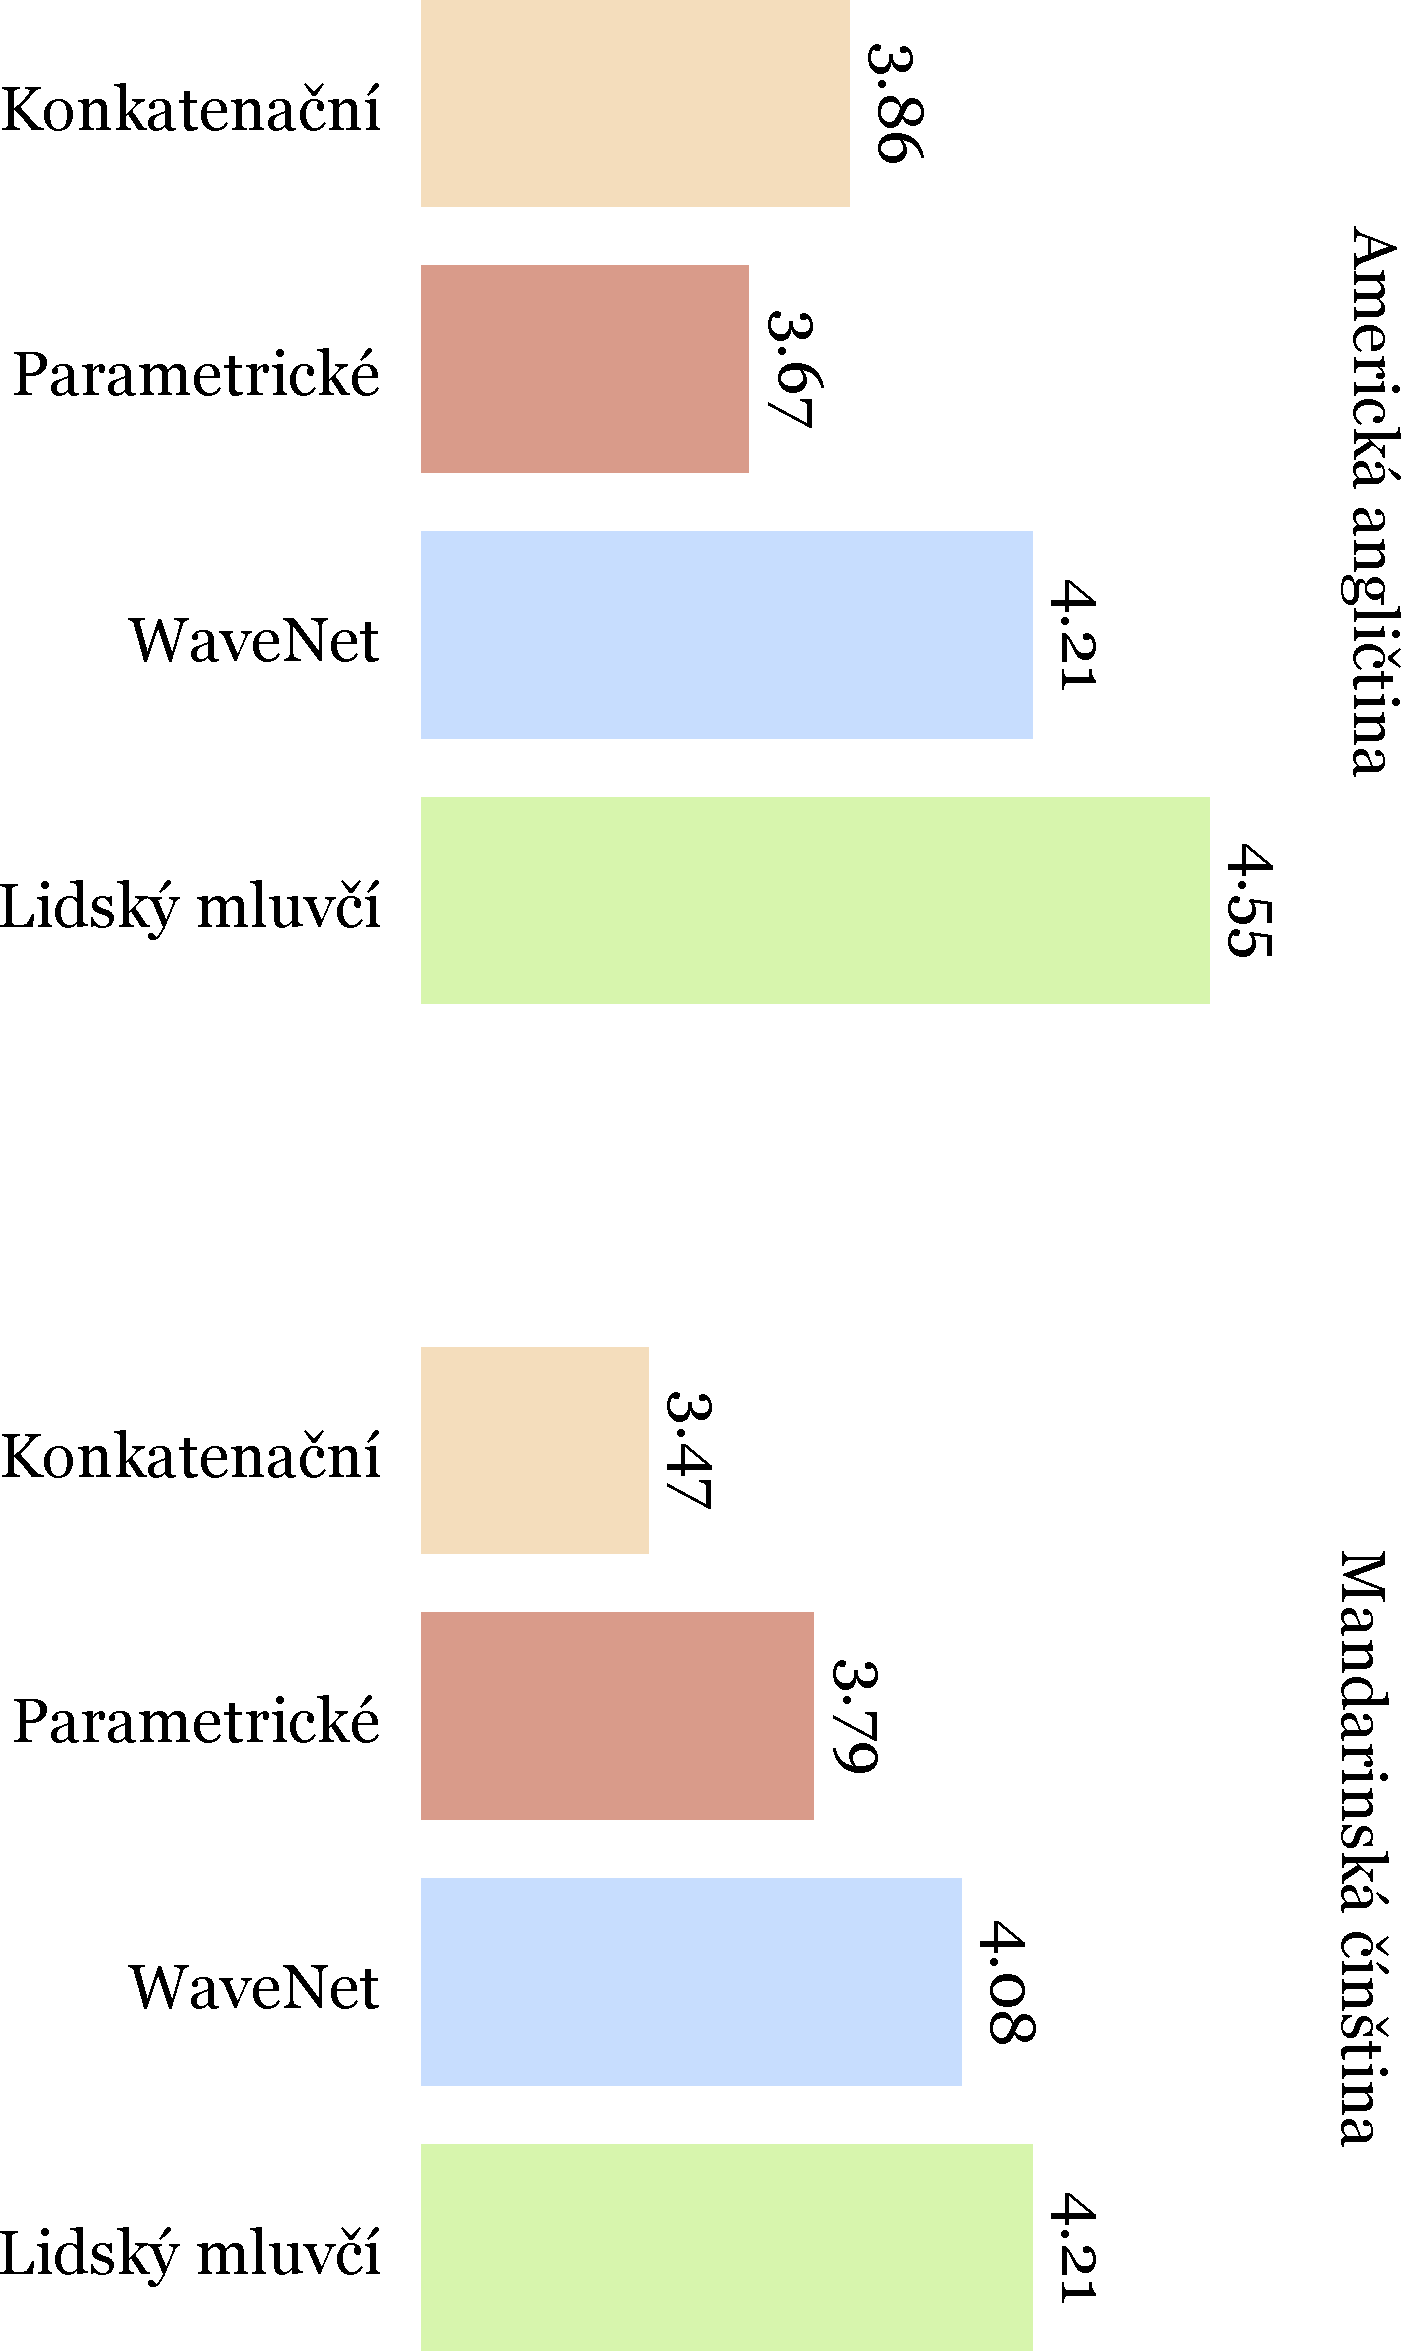
\includegraphics[angle=90, width=0.98\textwidth]{../img/wavenet-comparison.pdf}
    \caption{Porovnání průměrného hodnocení přirozenosti řeči na stupnici 1-5, převzato z~dokumentace
        \citet[upraveno a přeloženo autorem]{google_tts}.}\label{img-wavenet}
\end{figure}

\chapter{Konstrukce dialogových systémů}

Krátce shrneme dva
nejběžnější přístupy ke konstrukci. Tradiční je přístup, který bychom
mohli označit jako postupný. Taková konstrukce čítá několik komponent, kde
každá zajišťuje část práce nutné k porozumění uživateli a zodpovězení jeho
prohlášení. Ten uvedeme jako první, neboť dobře ilustruje, co všechno vlastně
člověk podvědomě při komunikaci dělá. Dále uvedeme tzv. \textit{end-to-end}
systémy využívající metod strojového učení, které umožňují nahrazení až
několika komponent jedním modelem. Tento přístup první uvedený v mnohém
předčil, ale je běžnou praxí obě konstrukce kombinovat.

TODO možná terminologie? spíš ne

\section{Tradiční inkrementální systémy}

Již jsme zmínili, že takové systémy mají několik komponent, které na sebe
navazují, jedna obvykle určitým způsobem využije výstup z předchozí jako svůj
vstup.

\subsection{Převod mluvené řeči na text}

Zkráceně značíme nejčastěji \textit{STT} z anglického \textit{speech-to-text}.
Jak název napovídá, úkolem této komponenty je převést zvukový projev na text.
Dříve byly k tomuto účelu využívány především \textit{skryté
    Markovovy modely (hidden Markov models, HMM)}. Tyto modely se nazývají skryté,
protože jejich vnitřní stavy nemohou být pozorovány, vidíme pouze výstup.
Jsou postaveny na \textit{Markovových řetězcích}, jejichž základním předpokladem
je, že v sekvenci stavů pravděpodobnost příštího závisí jen na stavu aktuálním,
nikoliv žádném předchozím, jak uvádí například \citet[strana 4]{brooks_handbook_2011}.
Jejich výhodou je, že jsou poměrně jednoduché a nenáročné na výpočetní výkon.

Jako v mnoha jiných odvětvích, i zde přišly ke slovu neuronové sítě, které HMM
ve většině směrů překonaly. V dobrých podmínkách jsou schopny provést přepis
téměř bezchybně. Opět však narážíme i na jejich slabé stránky,
totiž vysokou náročnost na množství trénovacích dat a výpočetní výkon.

O obecných problémech typu okolního hluku či různé výslovnosti jsme se
již zmiňovali. Zde ještě dodáme, že komplikací může být i nedostatečná kvalita
nahrávky. Mimo jiné z těchto důvodů výstupem často nebývá jen jedno
slovo či věta, nýbrž několik spolu s \textit{jistotou}, kterou model této
variantě přiřadil.

\subsection{Extrakce významu}

\subsubsection{Obecný význam}
Nyní když máme textovou reprezentaci výpovědi, budeme se z ní snažit nějak
jednoduššeji vyjádřit podstatné části. Této komponentě se obvykle říká
\textit{porozumění jazyku (natural language understanding, NLU)}. V jistém
smyslu je její úkol nejnáročnější, neboť jazyky mají mnoho nejasností,
víceznačností a nuancí obecně. Výstupem této komponenty je často opět
seznam reprezentací s hodnotou, nakolik si je systém tou konkrétní
interpretací jistý.

Jako onu jednodušší reprezentaci často používáme trojice
\textit{úmysl}--\textit{slot}--\textit{hodnota}. Pro ilustraci například
úryvek \uv{v deset hodin} bychom mohli přeložit na trojici
informovat--čas--10:00. K získání relevantních trojic můžeme využít ručně
psané \textit{regulární výrazy} vyhledávající vzorce v textu, tento přístup
je však dost náročný. Pro rozumnou funkcionalitu takových výrazů musíme napsat
stovky. Dnes obvykle lepší alternativou jsou opět modely využívající strojové
učení.

\subsubsection{Jména a názvy}
Důležitou součástí je \textit{rozpoznání jmenných entit} (anglicky
\textit{named entity recognition, NER}),
kde cílem je rozpoznat v textu názvy, které jako slova sama o sobě nemají
význam, pokud nevíme, že jde o název. Zajímají nás jak jména lidí, tak
geografických objektů či čehokoliv jiného, v závislosti na cílové doméně.

K jejich nalezení se opět často používají modely strojového učení, pro češtinu
jeden takový popsali \citet{ekstein_czech_2019}. Na pomoc či další zpracování
můžeme využít metriky vzdálenosti mezi textovými řetězci,
jako je \textit{Levenshteinova vzdálenost}, pravděpodobně představena autorem v
článku roku 1965 \citep{Levenshtein1965BinaryCC} . Ta říká, kolik nejméně úprav
musíme u jednoho řetězce udělat, abychom dostali druhý, tedy zjednoudšeně řečeno
jak moc jsou si dva řetězce podobné. Trochu problém nastává u krátkých slov,
protože u nich i velmi málo úpravami můžeme dostat slovo kompletně rozdílné.

\subsection{Zachování stavu}

Od systému samozřejmě budeme vyžadovat určitou paměť. Pokud řekneme, že
chceme někomu zavolat, pak dostaneme otázku komu, a pak ji zodpovíme, očekáváme,
že systém si bude ještě pamatovat, že chceme volat. Tato komponenta je
značena \textit{DST} z anglického \textit{Dialogue State Tracker}. V případě
zmíněné reprezentace pomocí trojic paměti docílíme obvykle tak, že si pro každý
slot pamatujeme hodnotu. Buď jednu, kterou v případě detekce jiné ihned přepíšeme,
nebo si pro každý slot pamatujeme pravděpodobnostní rozložení více hodnot, které
průběžně upravujeme. Téma hezky shrnují Williams, Raux a Handerson ve svém článku
\citep{williams_dialog_2016}. Paměť nesmíme zapomenout v určitých případech
resetovat, například když uživatel změní celý svůj cíl, jím dříve
zmíněné hodnoty se stávají irelevantními.

\subsection{Rozhodnutí o dalším kroku}

Máme uživatelovu aktuální výpověď a relevantní historii dialogu, nyní potřebujeme
rozhodnout, jak zareagujeme. Můžeme ručně napsat pravidla, na základě kterých
se rozhodneme o odpovědi. U systémů zaměřených na plnění úkolů je častou
strategií snaha zjistit uživatelův cíl a následné získání informací potřebných
k tomuto cíli (například pokud máme zarezervovat let, potřebujeme vědět kdy,
odkud a kam), jinými slovy vyplnění potřebných slotů. Rozhodovacích pravidel
však potřebujeme mnoho a zvláště u větších systémů může být výsledný proces dost
zmatený. I zde jsou dnes využívány statistické modely a různé druhy strojového
učení (hodí se zmínit především \textit{zpětnovazebné}). Výstupem této komponenty
bývá opět určitý mezistupeň, jednodušší reprezentace nesoucí význam. Využít
můžeme již zmíněné trojice úmysl--slot--hodnota.

\subsection{Vytvoření odpovědi v přirozeném jazyce}

Z interní reprezentace významu nyní potřebujeme vytvořit odpověď v přirozeném
jazyce, kterou pochopí libovolný uživatel. Můžeme využít \textit{šablon}, do
kterých doplníme vynechané části dle stavu dialogu (například
\uv{Přejete si odlétat [zítra] v [10:00]?}). Přidáním více variant (ze kterých
pak můžeme volit náhodně) pro každou šablonu dosáhneme i určité autentičnosti
dialogu. Opět narážíme na pracnost tohoto přístupu, šablon totiž i pro
jednotlivou doménu musíme vytvořit desítky a více. Přesto mohou posloužit až
překvapivě dobře. Dalšími možnostmi je použít formálních gramatik či i zde
strojového učení.

\subsection{Převod textu na hlas}

Obdobně jako u převodu opačným směrem, značíme \textit{TTS}. Důležitými pojmy
při popisu řeči jsou \textit{fón}, což je v zásadě jakýkoliv zvuk nehledě na
význam; a \textit{foném}, což je nejmenší část jazyka,
pomocí které jsme schopni význam rozlišit. Především jejich analýza pomáhá
při snaze o počítačovou syntézu hlasu.

Důkazem může být například
\textit{konkatenační} přístup ke generování hlasu, kdy nahrajeme mluvu člověka,
nahrávku rozdělíme na \textit{difóny} (dva za sebou jdoucí fóny) a ty pak
zpět \uv{slepíme} v požadovaném pořadí. V této základní variantě dostaneme
hlas, který bude znít značně roboticky (mimo jiné kvůli absenci intonace či
přízvuků), ale uživatel z něj dokáže pochopit význam. Při dostatečném množství
vzorových dat a aplikaci dalších vylepšení však dostáváme již velmi dobré
výsledky.

Mezi další využíváné přístupy patří opět využití HMM nebo strojového učení. Modely
využívající hluboké neuronové sítě jsou již pro některé jazyky téměř
nerozeznatelné od lidského mluvčího, když velmi dobře zvládají výslovnost,
intonaci i důrazy.

\section{End-to-end modely}


%%% Fiktivní kapitola s ukázkami tabulek, obrázků a kódu

\chapter{Tabulky, obrázky, programy}

Používání tabulek a grafů v~odborném textu má některá společná
pravidla a~některá specifická. Tabulky a grafy neuvádíme přímo do
textu, ale umístíme je buď na samostatné stránky nebo na vyhrazené
místo v~horní nebo dolní části běžných stránek. \LaTeX\ se o~umístění
plovoucích grafů a tabulek postará automaticky.

Každý graf a tabulku
očíslujeme a umístíme pod ně legendu. Legenda má popisovat obsah grafu
či tabulky tak podrobně, aby jim čtenář rozuměl bez důkladného
studování textu práce.

Na každou tabulku a graf musí být v~textu odkaz
pomocí jejich čísla. Na příslušném místě textu pak shrneme ty
nejdůležitější závěry, které lze z~tabulky či grafu učinit. Text by
měl být čitelný a srozumitelný i~bez prohlížení tabulek a grafů a
tabulky a grafy by měly být srozumitelné i~bez podrobné četby textu.

Na tabulky a grafy odkazujeme pokud možno nepřímo v~průběhu běžného
toku textu; místo \emph{\uv{Tabulka~\ref{tab03:Nejaka} ukazuje, že
    muži jsou v~průměru o~$9,9\,\rm kg$ těžší než ženy}} raději napíšeme
\emph{\uv{Muži jsou o~$9,9\,\rm kg$ těžší než ženy (viz
    Tabulka~\ref{tab03:Nejaka})}}.

\section{Tabulky}

\begin{table}[b!]

\centering
%%% Tabulka používá následující balíčky:
%%%   - booktabs (\toprule, \midrule, \bottomrule)
%%%   - dcolumn (typ sloupce D: vycentrovaná čísla zarovnaná na
%%%     desetinnou čárku
%%%     Všimněte si, že ve zdrojovém kódu jsou desetinné tečky, ale
%%%     tisknou se čárky.
%%% Dále používáme příkazy \pulrad a \mc definované v makra.tex

\begin{tabular}{l@{\hspace{1.5cm}}D{.}{,}{3.2}D{.}{,}{1.2}D{.}{,}{2.3}}
\toprule
 & \mc{} & \mc{\textbf{Směrod.}} & \mc{} \\
\pulrad{\textbf{Efekt}} & \mc{\pulrad{\textbf{Odhad}}} & \mc{\textbf{chyba}$^a$} &
\mc{\pulrad{\textbf{P-hodnota}}} \\
\midrule
Abs. člen     & -10.01 & 1.01 & \mc{---} \\
Pohlaví (muž) & 9.89   & 5.98 & 0.098 \\
Výška (cm)    & 0.78   & 0.12 & <0.001 \\
\bottomrule
\multicolumn{4}{l}{\footnotesize \textit{Pozn:}
$^a$ Směrodatná chyba odhadu metodou Monte Carlo.}
\end{tabular}

\caption{Maximálně věrohodné odhady v~modelu M.}\label{tab03:Nejaka}

\end{table}

U~\textbf{tabulek} se doporučuje dodržovat následující pravidla:

\begin{itemize} %% nebo compactitem z balíku paralist
\item Vyhýbat se svislým linkám. Silnějšími vodorovnými linkami
  oddělit tabulku od okolního textu včetně legendy, slabšími
  vodorovnými linkami oddělovat záhlaví sloupců od těla tabulky a
  jednotlivé části tabulky mezi sebou. V~\LaTeX u tuto podobu tabulek
  implementuje balík \texttt{booktabs}. Chceme-li výrazněji oddělit
  některé sloupce od jiných, vložíme mezi ně větší mezeru.
\item Neměnit typ, formát a význam obsahu políček v~tomtéž sloupci
  (není dobré do téhož sloupce zapisovat tu průměr, onde procenta).
\item Neopakovat tentýž obsah políček mnohokrát za sebou. Máme-li
  sloupec \textit{Rozptyl}, který v~prvních deseti řádcích obsahuje
  hodnotu $0,5$ a v~druhých deseti řádcích hodnotu $1,5$, pak tento
  sloupec raději zrušíme a vyřešíme to jinak. Například můžeme tabulku
  rozdělit na dvě nebo do ní vložit popisné řádky, které informují
o~nějaké proměnné hodnotě opakující se v~následujícím oddíle tabulky
  (např. \emph{\uv{Rozptyl${}=0,5$}} a níže \emph{\uv{Rozptyl${}=
      1,5$}}).
\item Čísla v~tabulce zarovnávat na desetinnou čárku.
\item V~tabulce je někdy potřebné používat zkratky, které se jinde
nevyskytují. Tyto zkratky můžeme vysvětlit v~legendě nebo
v~poznámkách pod tabulkou. Poznámky pod tabulkou můžeme využít i
k~podrobnějšímu vysvětlení významu  některých sloupců nebo hodnot.
\end{itemize}

\section{Obrázky}

Několik rad týkajících se obrázků a grafů.

\begin{itemize}
\item Graf by měl být vytvořen ve velikosti, v~níž bude použit
  v~práci. Zmenšení příliš velkého grafu vede ke špatné čitelnosti
  popisků.
\item Osy grafu musí být řádně popsány ve stejném jazyce, v~jakém je
  psána práce (absenci diakritiky lze tolerovat). Kreslíme-li graf
  hmotnosti proti výšce, nenecháme na nich popisky \texttt{ht} a
  \texttt{wt}, ale osy popíšeme \emph{Výška [cm]} a~\emph{Hmotnost
    [kg]}. Kreslíme-li graf funkce $h(x)$, popíšeme osy $x$ a $h(x)$.
  Každá osa musí mít jasně určenou škálu.
\item Chceme-li na dvourozměrném grafu vyznačit velké množství bodů,
  dáme pozor, aby se neslily do jednolité černé tmy. Je-li bodů mnoho,
  zmenšíme velikost symbolu, kterým je vykreslujeme, anebo vybereme
  jen malou část bodů, kterou do grafu zaneseme. Grafy, které obsahují
  tisíce bodů, dělají problémy hlavně v~elektronických dokumentech,
  protože výrazně zvětšují velikost souborů.
\item Budeme-li práci tisknout černobíle, vyhneme se používání barev.
  Čáry roz\-li\-šu\-je\-me typem (plná, tečkovaná, čerchovaná,\ldots), plochy
  dostatečně roz\-díl\-ný\-mi intensitami šedé nebo šrafováním. Význam
  jednotlivých typů čar a~ploch vysvětlíme buď v~textové legendě ke
  grafu anebo v~grafické legendě, která je přímo součástí obrázku.
\item Vyhýbejte se bitmapovým obrázkům o~nízkém rozlišení a zejména
  JPEGům (zuby a kompresní artefakty nevypadají na papíře pěkně).
  Lepší je vytvářet obrázky vektorově a vložit do textu jako PDF.
\end{itemize}

\section{Programy}

Algoritmy, výpisy programů a popis interakce s~programy je vhodné
odlišit od ostatního textu. Jednou z~možností je použití {\LaTeX}o\-vé\-ho balíčku
\texttt{fancyvrb} (fancy verbatim), pomocí něhož je v~souboru \texttt{makra.tex}
nadefinováno prostředí \texttt{code}. Pomocí něho lze vytvořit
např. následující ukázky.

\begin{code}
> mean(x)
[1] 158.90
> objekt$prumer
[1] 158.90
\end{code}
%$
Menší písmo:
\begin{code}[fontsize=\footnotesize]
> mean(x)
[1] 158.90
> objekt$prumer
[1] 158.90
\end{code}
%$
Bez rámečku:
\begin{code}[frame=none]
> mean(x)
[1] 158.90
> objekt$prumer
[1] 158.90
\end{code}
%$
Užší rámeček:
\begin{code}[xrightmargin=20em]
> mean(x)
[1] 158.90
> objekt$prumer
[1] 158.90
\end{code}
%$

\begin{figure}[p]\centering
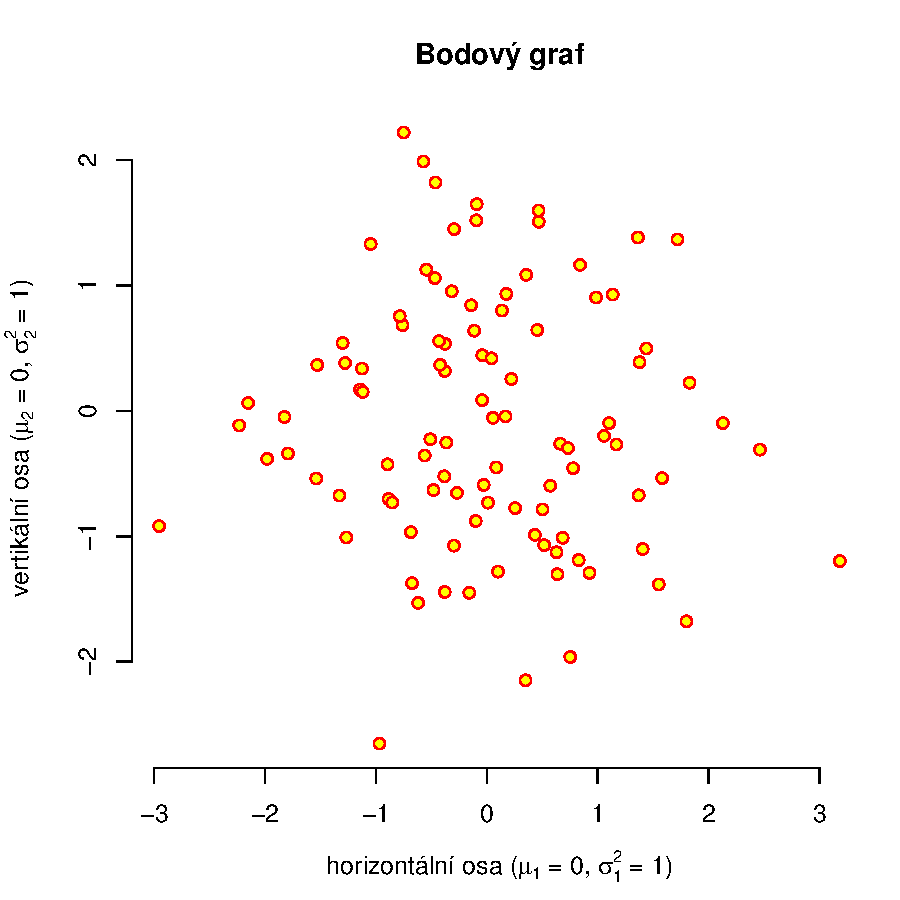
\includegraphics[width=140mm, height=140mm]{../img/ukazka-obr01}
% Příponu není potřeba explicitně uvádět, pdflatex automaticky hledá pdf.
% Rozměry také není nutné uvádět.
\caption{Náhodný výběr z~rozdělení $\mathcal{N}_2(\boldsymbol{0},\,I)$.}
\label{obr03:Nvyber}

\end{figure}

\begin{figure}[p]\centering
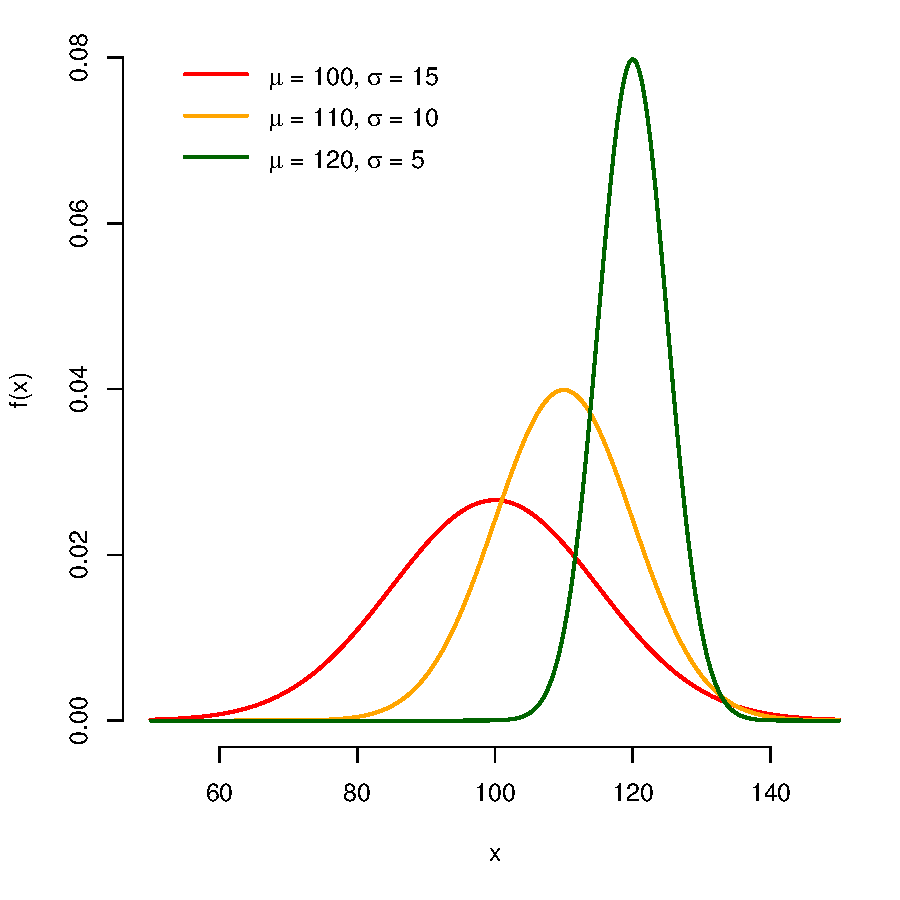
\includegraphics[width=140mm, height=140mm]{../img/ukazka-obr02}
\caption{Hustoty několika normálních rozdělení.}
\label{obr03:Nhust}
\end{figure}

\begin{figure}[p]\centering
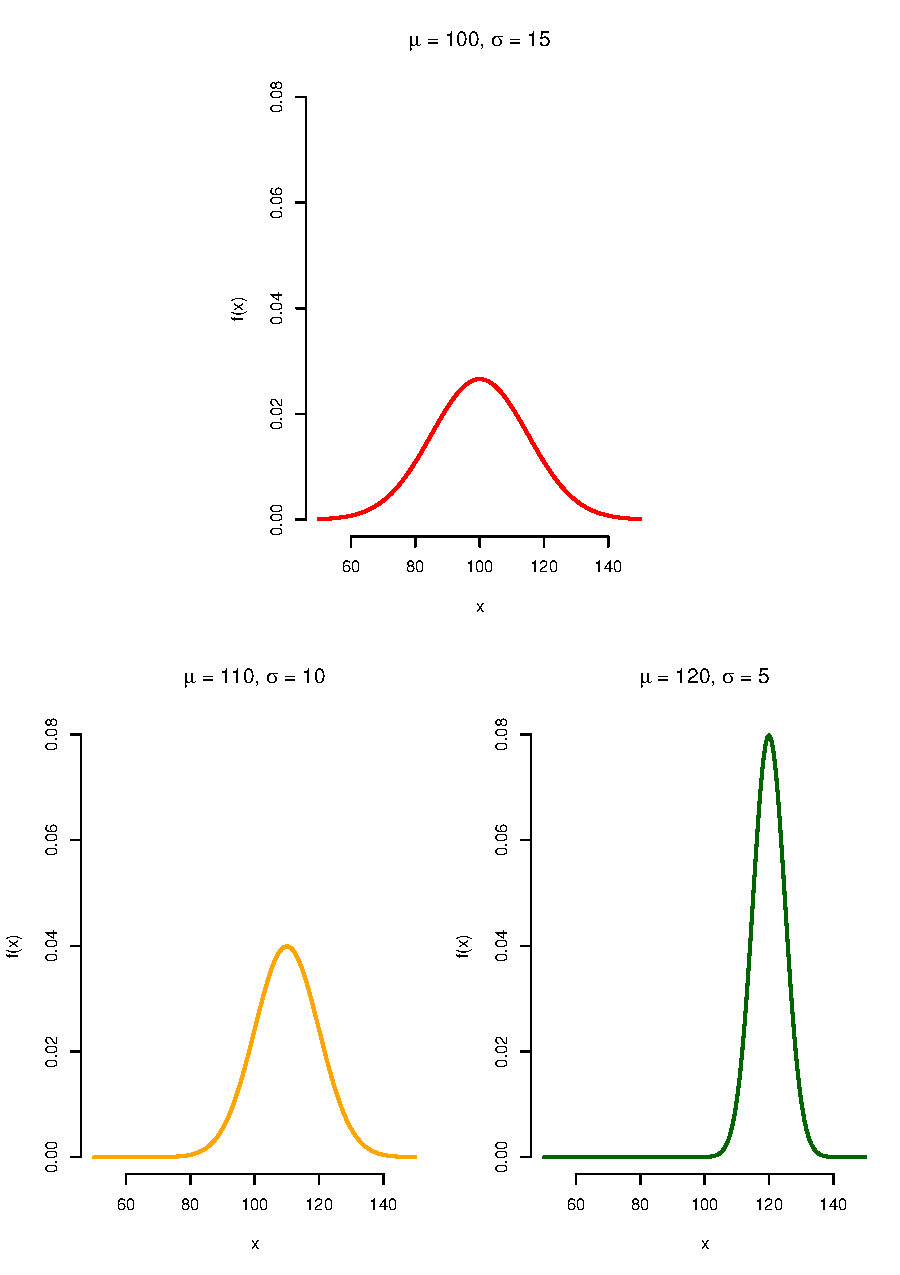
\includegraphics[width=140mm, height=198mm]{../img/ukazka-obr03}
\caption{Hustoty několika normálních rozdělení.}
\label{obr03:Nhust:podruhe}

\end{figure}

\chapter{Implementace}

V úvodu této kapitoly popíšeme koncepci programu, co kde
běží a jakým způsobem spolu komunikuje. Následně v sekci~\ref{analysis}
rozebereme zvolenou platformu a programovací jazyky,
další sekce budou pak věnovány popisu komponent, které jsme museli
naimplementovat pro funkci celého systému. Konkrétně jde o aplikaci pro
mobilní telefony s operačním systémem Android (v sekci~\ref{app}), vytvoření instance WA pro řízení
dialogu (s popisem získání nejběžnějších českých jmen pro trénink, \ref{wainit}) a komponenty
pro porovnání entit nalezených pomocí WA se seznamem kontaktů (\ref{matching}).

Jak jsme již uvedli, výsledkem je z uživatelského pohledu mobilní
aplikace. Většina vnitřních procesů však probíhá v cloudu, aplikace
je jen jakýmsi spojem a médiem pro komunikaci s uživatelem. Celý běh
je znázorněn na obrázku~\ref{img-flowchart}. Stisknutím tlačítka v
telefonu se
inicializuje session ve WA běžícím v cloudu IBM a spustí rozpoznávání řeči,
které běží na serverech Google. Po zahájení session ve WA jsou tam též
odeslána jména kontaktů uložených v telefonu. Jakmile je z hlasu rozpoznán
text, je vrácen zpět do aplikace a odtud odeslán jako zpráva do WA.
Ten rozhodne, zda je potřeba volat
porovnávací komponentu. Pokud ano, zavolá ji z jiné části IBM cloudu,
předá jí relevantní data a získá od ní odpověď. V každém případě
WA vygeneruje odpověď na zaslanou zprávu a odešle ji zpět do telefonu.
Tam je odpověď z WA zpracována (mj. je rozhodnuto, zda by měl být
zahájen hovor) a odeslána do syntetizátoru řeči na servery Google.
Odtud je hlas k přehrání vrácen zpět do aplikace, tam je přehrán
a následně je na základě dřívějšího rozhodnutí buď spuštěno znovu
rozpoznání hlasu, nebo je zahájen hovor a aplikace ukončena.


\begin{figure}[h]\label{img-flowchart}
    \centering
    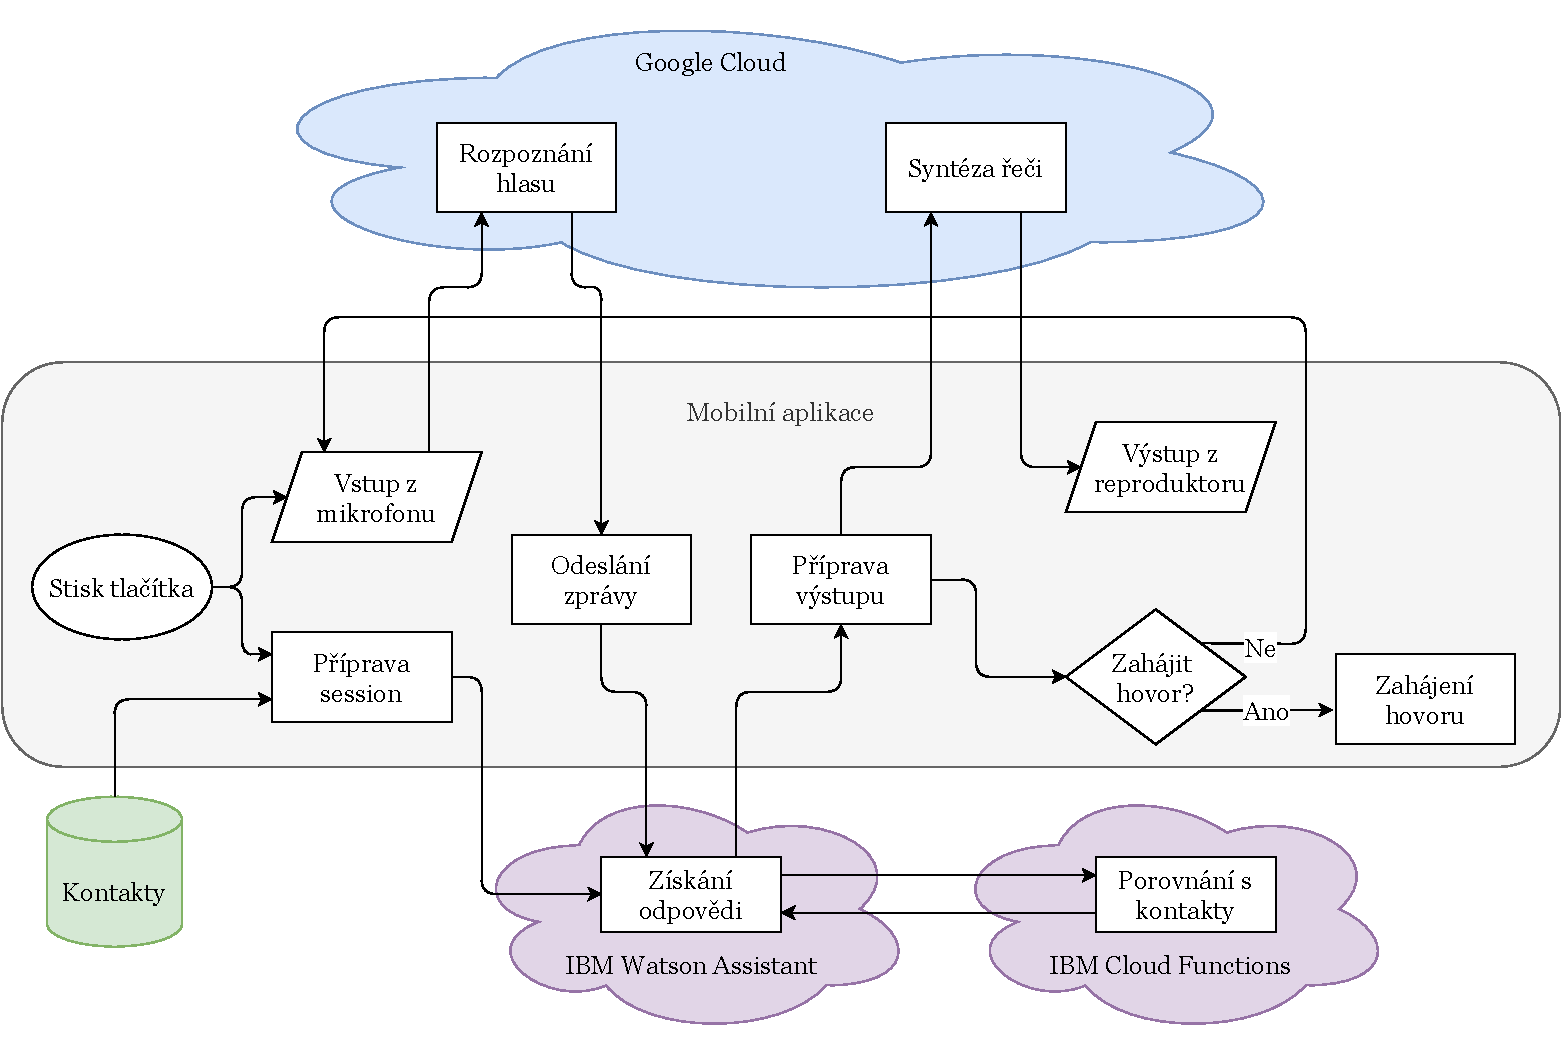
\includegraphics[width=0.98\textwidth]{../img/app-flowchart.pdf}
    \caption{Nákres fungování celého systému}
\end{figure}

\section{Platforma a programovací jazyky}\label{analysis}

\subsection{Platforma a jazyk mobilní aplikace}
Pro mobilní aplikace máme v dnešní době v zásadě dvě možnosti, iOS nebo Android.
Zvolili jsme Android, neboť je celkově otevřenější, autor telefon s tímto
operačním systémem vlastní a mají tedy alespoň uživatelské zkušenosti. IBM navíc
poskytuje vývojový balíček (\textit{SDK}) pro použití WA v programovacím
jazyku Java, který je použitelný i v Androidu.

Z hlediska programovacího jazyka padla volba na Kotlin. Existují různé frameworky
schopné zkompilovat pro Android program psaný téměř v libovolném programovacím
jazyce, ale většina nakonec musí používat nějakou další překladovou vrstvu.
Kotlin je jeden z jazyků, ve kterém lze psát nativní aplikace pro Android. Programy
v něm napsané lze totiž zkompilovat pro spuštění v \textit{JVM} (\textit{Java Virtual Machine}),
toto prostředí popisuje \citet{prof_tejinder_singh_hotspot_2014}.
Kotlin dokonce umožňuje interoperabilitu s Javou, což umožnilo
využití zmíněného SDK. Jeho výhoda oproti Javě je, že je celkově modernější,
psaní a čtení programů v něm je díky přehlednější syntaxi jednodušší a kratší,
navíc je doporučený samotnou firmou Google jakožto vedoucím vývoje operačního
systému Android \citep{android_blog}.
Další vlastností, na kterou při výběru nebyl brán tak velký
zřetel, ale nakonec se ukázala jako relativně zásadní, je podpora \textit{koprogramů}
(\textit{coroutines}), jejichž možnou implementaci ukazují \citet{theory_practice_coroutines}.

\subsection{Volba asistenta a jeho inicializace}
Frameworků pro tvorbu asistentů existuje na trhu mnoho, jen jeden však aktuálně oficiálně plně
podporuje český jazyk -- Watson Assistant od IBM. Proto zde volba jednoduše
padla právě na něj.

Inicializace WA lze provést v interaktivním prostředí v prohlížeči. Toto
prostředí je však v mnohém omezené. V našem případě jsme například potřebovali
vložit stovky entit pro trénování rozpoznání. Přenést je do WA přes prohlížeč
by bylo absurdně náročné, navíc složitě replikovatelné. Použili jsme proto opět
po SDK, pomocí kterého můžeme WA iniciovat relativně krátkým skriptem. Na volbě
konkrétního programovacího jazyka zde téměř nezáleželo (skript je krátký a běží
jen jednou pro inicializaci), zvolili jsme proto Python jakožto dobře čitelný
jazyk, se kterým máme mnoho zkušeností.

\subsection{Jazyk a prostředí běhu porovnávací komponenty}

Volba jazyka byla zde také jednoduchá, kolegové z MAMA AI totiž plánovali
komponentu také využít a požadovaným jazykem byl Python. To bylo z naší
strany naprosto v pořádku, protože k tomuto jazyku máme blízko a nepředstavoval
pro toto použití žádné výraznější limitace.

Při implementaci jsme potřebovali počítat podobnost řetězců. Algoritmus
pro tento výpočet je relativně komplikovaný a běžně používaný, nedávalo tedy
smysl programovat jej znovu. Využili jsme modul
\texttt{editdistance}\footnote{\url{https://pypi.org/project/editdistance/}},
protože je psaný v rychlejším jazyce C++ a má vhodnou licenci.

Dále bylo potřeba vyřešit, kde tato komponenta poběží. Nakonec jsme vybrali
službu IBM Cloud Functions. Původním nápadem bylo
zprovoznění webového serveru, který by vyřizoval požadavky na tuto komponentu.
To by však vyžadovalo další kód pro správu a především hardware, na kterém by
tento server běžel. Při hledání alternativ jsme dostali doporučení na
\textit{funkce poskytované jako služby} (\textit{function as a service, FaaS}),
které nabízí většina větších poskytovatelů cloudů. Jednoduše řečeno, na daný
server lze nahrát kód, který přijímá a vrací (obvykle) soubory formátu JSON a
běží jen ve chvíli, kdy dostane nějaký požadavek. Liší se tak od standardních
webových serverů, které musí \uv{poslouchat} neustále. Konkrétně byla vybrána
služba IBM Cloud Functions především proto, že lze spravovat ze stejného účtu jako
WA. Teoreticky může být výhoda využití stejného poskytovatele ještě v tom, že
servery budou na stejném místě a tedy výměna dat mezi nimi bude probíhat rychleji.

\section{Mobilní aplikace}\label{app}

Pro vytvoření aplikace jsme využili integrované vývojové prostředí
\textit{Android Studio}. Původním záměrem bylo využít \textit{Visual Studio Code}
spolu s \textit{vývojovými kontejnery} za použití virtualizačního softwaru
\textit{Docker}, především díky přenositelnosti a relativní nenáročnosti
na výpočetní výkon. Ukázalo se však, že tato cesta není při vývoji aplikací
pro Android v jazyce Kotlin pod operačním systémem Windows úplně běžná a
naráží na mnoho komplikací, tedy je především pro začátek silně nevhodná.
Pro kompilaci využíváme běžně používaný \textit{gradle}.

Aplikace musela vyřešit několik věcí: získání oprávnění ke všem operacím,
získání kontaktů uživatele, vytvoření \textit{session} ve WA a odeslání
jmen kontaktů, spuštění rozpoznání hlasu, po dokončení jeho výsledek odeslat
jako zprávu do WA, po získání odpovědi spustit hlasový syntetizátor, po skončení
jeho projevu buď spustit rozpoznání hlasu a celý běh znovu, nebo zahájit
hovor. Všemi součástmi se budeme zabývat v následujících podsekcích, začneme
ale celkovou koncepcí a vzhledem.

\subsection{Celková koncepce a vzhled}

Jednotlivé komponenty (obvykle reprezentované jednou obrazovkou)
se v aplikacích
pro Android nazývají \textit{Activity}. Protože primárním způsobem interakce
s aplikací má být hlas, cílili jsme na jednoduché a sebevysvětlující grafické
rozhraní. Zvolili jsme tlačítko se symbolem mikrofonu na černém pozadí,
jak ukazuje obrázek~\ref{img-ui}. Tímto tlačítkem je zahájen dialog (v případě
dostatečných oprávnění, jejichž získání řešíme dále).

\begin{figure}[h]\label{img-ui}
    \centering
    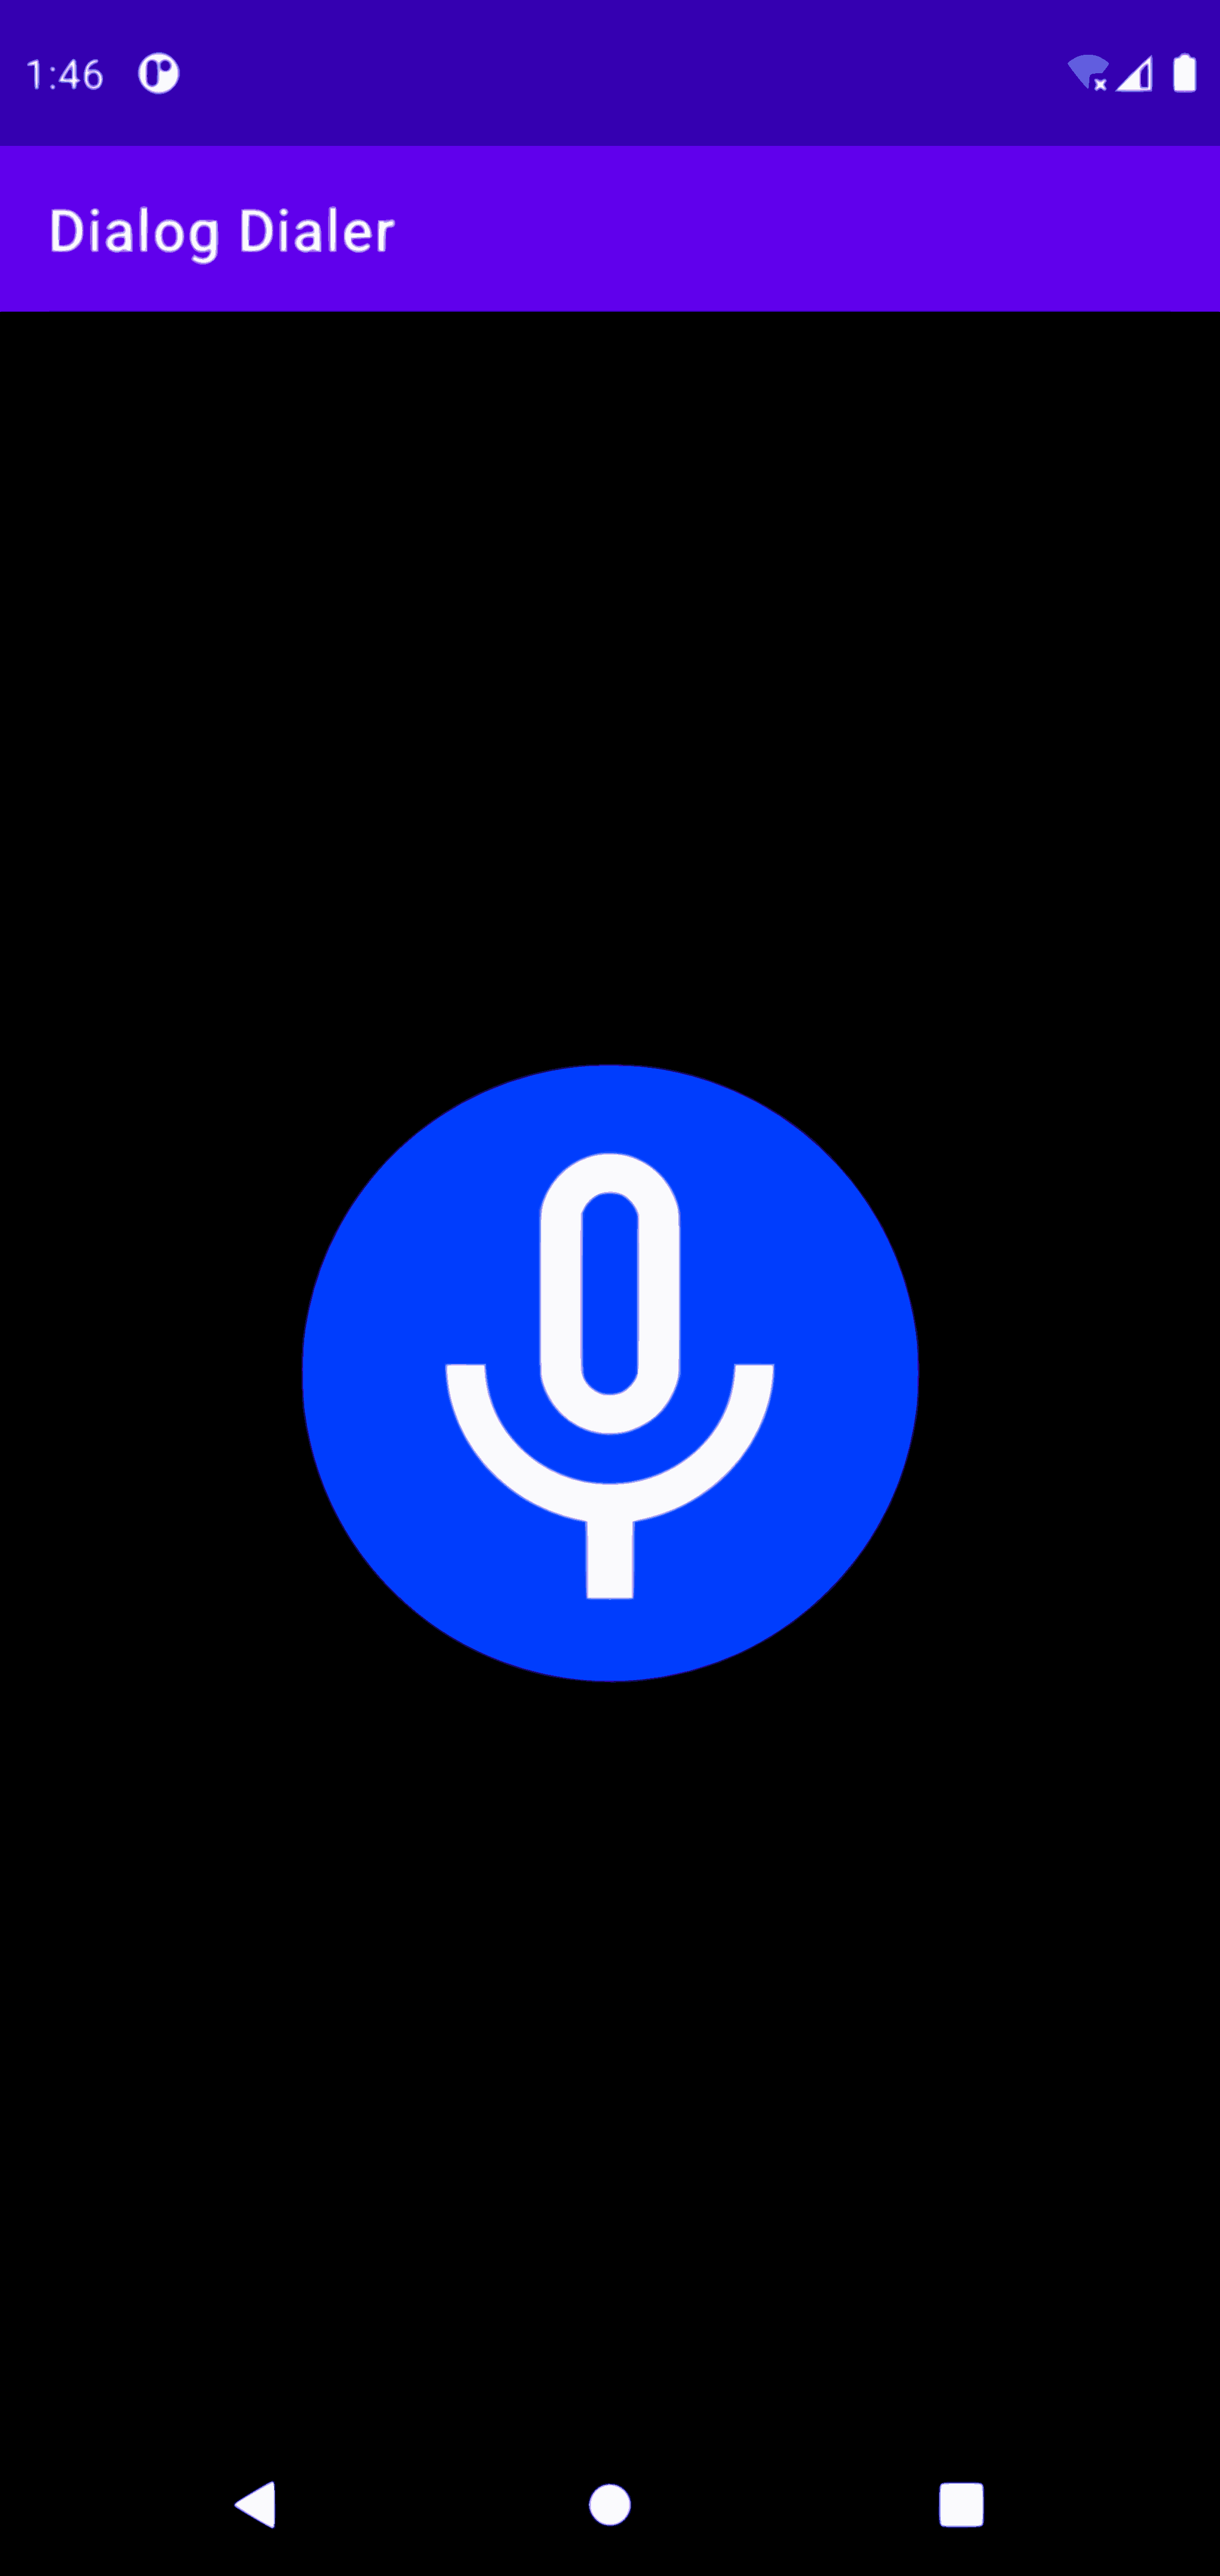
\includegraphics[width=0.3\textwidth]{../img/ui.pdf}
    \caption{Jednoduché uživatelské rozhraní}
\end{figure}

Protože nám stačí jedna obrazovka, je celý kód umístěn v jednom souboru
\texttt{MainActivity.kt}. Pro změnu grafického rozhraní z kódu je třeba
jejich propojení, které zajišťuje instance třídy \texttt{ActivityMainBinding}.
Toto je aktuálně oficiálně doporučený postup (na úkor dříve používaného
vyhledání pomocí \texttt{id}), ale vygenerování propojovací třídy musíme
povolit v souboru \texttt{build.gradle} na úrovni modulu.

Tato instance je využita při otevření aplikace pro \uv{nafouknutí} grafického
rozhraní a následně v kódu kdykoliv chceme k rozhraní přistupovat. To v našem
případě znamená nastavení reakce na stisk tlačítka, případně jeho deaktivace
či změna vzhledu pro indikaci probíhajících procesů.

\subsection{Získání oprávnění}

Pro svou správnou funkci potřebuje aplikace povolení nahrávat zvuk, číst
kontakty, vykonávat hovory a přistupovat k internetu. Všechna požadovaná
oprávnění musí být uvedena v souboru \texttt{AndroidManifest.xml}, první
tři jsou navíc oprávněními za času běhu, tedy o ně musíme explicitně
požádat. Oprávnění k přístupu k internetu není tak zásadní (především
protože neoperuje s uživatelovými daty), tedy je v Androidu automaticky
uděleno při instalaci aplikace.

Aktuálně oficiálně doporučeným postupem (který z toho důvodu využíváme), jak
řešit oprávnění, je nejprve o ně požádat, pokud uživatel odmítne a pokusí se
aplikaci znovu použít, zobrazit vysvětlení, k čemu jsou nutná a znovu o ně
požádat, a pokud znovu odmítne, již jen ukazovat upozornění o nedostupnosti.

Pro požádání o oprávnění potřebujeme spustit jinou aktivitu (pro získání
oprávnění existuje jedna vestavěná), vyčkat na její výsledek a na základě
něj rozhodnout o dalších krocích. K tomu využíváme opět aktuálně doporučenou
metodu \texttt{registerForActivityResult}. Pro zobrazení vysvětlení potřeby
oprávnění i upozornění o nedostupnosti využíváme třídu \texttt{AlertDialog}.

\subsection{Získání kontaktů}

Kontakty potřebujeme získat z úložiště telefonu, které se chová podobně jako
databáze. Proto dotaz na ně začneme na začátku inicializace celé služby WA
asynchronně jako koprogram. V rámci něj pak získáme jména a čísla kontaktů,
které uložíme do slovníku.

\subsection{Vytvoření session ve WA a odeslání jmen kontaktů}

Po začátku dotazu na kontakty vytvoříme instanci třídy \texttt{Assistant}
pro komunikaci s WA API, které předáme potřebné parametry a následně pošleme
požadavek pro zahájení session. V Androidu není možné posílat síťové požadavky
v hlavním vlákně (protože je potřeba udržovat ho volné pro UI), takže s výhodou
opět použijeme běh jako koprogram. Následně pomocí \texttt{await} zajistíme
kontrolu dokončení získávání kontaktů a předáme je jako \textit{kontext} do
WA session. Pokud se v průběhu něco nepovede, výjimku odchytíme a příště
se pokusíme provést celou inicializaci znovu.

Původní záměr byl odesílat kontakty do WA jako standardní zprávu, jenže
tam jsme brzy narazili na limit velikosti požadavku 2048 znaků. Delší
seznam kontaktů se do tohoto limitu nevejde, proto jsme nakonec využili
nastavení kontextu.

Důležité je ještě zmínit, že parametry pro komunikaci s WA jsou uloženy
zvlášť v souboru \texttt{credentials.xml}.

\subsection{Spuštění rozpoznávání hlasu}

Obdobně jako u získání
oprávnění potřebujeme spustit nějakou aktivitu a získat její výsledek, tedy
využijeme \texttt{registerForActivityResult}, tentokrát nejde o vestavěnou
aktivitu, ale můžeme využít parametr \texttt{Intent} (úmysl) při spuštění.
Protože ho potřebujeme používat často, vytvoříme ho jen jednou při otevření
aplikace a předáme mu potřebné parametry (český jazyk, jeden výsledek, atp.).
Když aktivita spuštěná s tímto úmyslem skončí, zkontrolujeme, že proběhla
úspěšně a pokračujeme k dalšímu kroku.

\subsection{Odeslání do WA a získání odpovědi}
Opět pomocí \texttt{await} vyčkáme nachystání WA. Pokud je vše připraveno,
pošleme v koprogramu (jedná se o síťový požadavek) text do WA a získáme odpověď.
Tuto odpověď ještě zpracujeme, pokud je na prvním řádku \texttt{[call]}, jedná
se o pokyn k hovoru, na druhém řádku najdeme jméno kontaktu a na třetím text k
přečtení. Pomocí jména kontaktu zjistíme jeho číslo, vytvoříme \texttt{Intent}
volání a nastavením proměnné \texttt{launchAgain} na \texttt{false} uložíme,
že dialog skončil. V opačném případě pošleme celou odpověď k přečtení.

\subsection{Spuštění hlasového syntetizátoru}

Převod textu na řeč budeme také potřebovat používat často, proto instanci
třídy \texttt{TextToSpeech} též vytvoříme při otevření programu. Nastavíme
ji na český jazyk a přepíšeme v ní funkci \texttt{onDone}, která je spuštěna,
když skončí přehrávání hlasu. Pokud dialog neskončil, spustíme celý běh
od rozpoznání hlasu zabalený ve funkci \texttt{launchPipeline} znovu. Pokud
skončil, jsme připraveni začít volat, vytočíme tedy číslo a ukončíme session ve
WA i celou aplikaci.

\section{Inicializace WA}\label{wainit}

Bohužel samotné vytvoření instance WA zatím není možné provést pomocí skriptů,
musíme ho tedy vytvořit ve webovém rozhraní. Odsud také získáme soubor
\texttt{ibm-credentials.env}, který budeme používat k autentizaci skriptů.

Když toto uděláme, jako první musíme vytvořit \textit{workspace}
(prostředí pro danou schopnost WA), což uděláme
jednoduchým požadavkem, který bude obsahovat parametry jako jméno nebo jazyk.
Zpět dostaneme odpověď, jejíž součástí bude \texttt{workspace\_id}, které budeme
dál potřebovat k manipulaci s prostředím. Pro úpravu tohoto prostředí
vždy budeme používat metodu \texttt{update\_workspace}, pomocí které můžeme
nahrát větší množství úprav naráz a nebudeme tak mít problémy s limitem na
počet požadavků.

\subsection{Úmysly a entity}

Jako první do něj přidáme detekci uživatelových úmyslů (intents), jejichž využití
jsme si představili v podsekci~\ref{nlu}. Zásadní je úmysl
\texttt{dial}, pomocí kterého detekujeme, že uživatel chce někomu volat. Pro
každý úmysl přidáme několik vzorových vět, na základě kterých by ho měl WA
rozpoznat. Ty jsou interně použity pro trénink umělé modelu stojícího za WA.
Obdobně vytvoříme zbývající úmysly \texttt{greet} a \texttt{bye}, aby náš
asistent uměl slušně pozdravit.

Jediné entity, které potřebujeme rozeznávat, jsou jména lidí, případně příjmení.
Do WA je k tréninku dostaneme obdobně jako úmysly. Uvažovali jsme, jak ale tato
data získat. Nakonec jsme využili data četnosti jmen a příjmení MVČR z roku 2017.
Sice již přímo na stránkách MVČR nejsou dostupná, ale ve ve webových archivech
existují. Tato data byla uložena ve formátu \texttt{xls} ve více listech, pro
počítačové zpracování ne moc ideálním. Pomocí knihovny \texttt{pandas} jsme je
tedy převedli do formátu \texttt{csv}, kde byla i výrazně menší. Následně jsme
vybrali všechna jména i příjmení, která v Česku k roku 2017 nosilo alespoň
200 (TODO check hranice) lidí a ta jsme nahráli do WA.

\subsection{Stavba dialogu}

Nejkomplikovanější částí bylo samotné sestavení průběhu dialogu s odesláním
dat do porovnávací komponenty. (TODO možná přesunout do popisu WA?) WA využívá
\textit{stromovou} reprezentaci dialogu,
kde sekvenčně kontrolujeme splnění podmínky (detekci úmyslu nebo entity) v
jednotlivých sourozencích. Jakmile v jednom najdeme podmínku splněnou, vybereme
odpověď z něj a pokud nějaké má, zanoříme se do jeho synů. Ve webovém rozhraní je
stavba dialogového stromu relativně přímočará, ale v některých místech omezená,
proto jsme i zde použili skript.

Vytváření dialogového stromu ve WA pomocí Python SDK je poněkud komplikovanější
než přes webové rozhraní. Například pokud chceme, aby vrchol vyžadoval zaplnění
určitého slotu a rozpoznanou hodnotu v něm ukládal do kontextu, musíme pro
každou tuto operaci vyrobit jeden podvrchol, zatímco v rozhraní bychom jen
vyplnili dvě pole.

Celkově je povrchová koncepce stromu relativně jednoduchá. Máme sourozenecké
vrcholy pro detekci uživatelových úmyslů pozdravit, zavolat a rozloučit se, navíc
dva speciální. Ty zajistí, že na začátku dialogu asistent nic neříká, a že
pokud není detekován žádný úmysl, asistent se na něj zeptá. Jediným vrcholem
s potomky je vrchol detekující úmysl volat, který ještě kontroluje zaplnění slotu
pro jméno (případně se na něj doptá). Nepřišli jsme na to, jak přímo z něj
uložit vstup a rozpoznané entity do kontextu, proto jeho syn dělá právě to. Ten
má dalšího syna, který relevantní kontext (vstup, rozpoznané entity a kontakty)
odešle do \textit{webhooku} (v zásadě webová adresa očekávající vstup a vracející
výstup, oboje ve formátu JSON), kde běží porovnávací komponenta. Získá tak její
výstup a na základě něj generuje odpověď -- pokud dostal zpět jedno jméno,
vyzve k zahájení hovoru; pokud více, vyzve k vybrání (a nastaví je do kontextu,
aby příště bylo porovnáváno jen s nimi); pokud žádné, oznámí že nic neodpovídá.
Poté se vrátí do uzlu připravujícího údaje, aby mohlo být provedeno případné
upřesnění.

TODO možná obrázek stromu?

\section{Porovnávací komponenta}\label{matching}

Tuto komponentu jsme implementovali pro obecné použití v dialogových systémech
v rámci knihovny \texttt{mConversation} MAMA AI, součástí jsou desítky testů
využívající frameworku \texttt{pytest}. Za účelem využití v aplikaci jsme komponentu
drobně upravili pro kontext vybírání z telefonního seznamu. Proto zde první popíšeme
obecnou část cílů a implementace, a pak konkrétní provedené úpravy.

Vstupem komponenty jsou entity rozpoznané pomocí WA, původní textový vstup do něj
a určitý (obvykle vázaný na uživatele) seznam entit. Cílem je vybrat entitu ze seznamu,
která nejvíce odpovídá vstupu do WA. V úvahu přitom nejsou brány jen entity, které
WA rozpoznal, ale i originální vstup. Pokud tak například uživatel zmíní běžné jméno a
neběžné příjmení, a WA rozpozná jako entitu jen jméno, komponenta dokáže najít a využít
i příjmení, takže pravděpodobně vrátí pouze jeden kontakt. Kdyby ho v úvahu nevzala,
vrátí všechny kontakty odpovídající jménu (s jinými příjmeními).

Součástí je i příprava pro určité rozšíření využívající strojového učení -- každý
uživatel by měl mít uložený svůj model, který se naučí jeho preference a bude se
průběžně zlepšovat využitím zpětné vazby. To je ale zatím jen koncept.

\subsection{Předzpracování}

K seznamu kontaktů si vytvoříme slovník,
který jako klíče bude mít všechny části kontaktů a jako hodnoty indexy do původního
seznamu. Tedy například pokud máme v seznamu na prvním místě kontakt \uv{Jan Novák},
ve slovníku budou \uv{Jan} i \uv{Novák} odkazovat na index 1.

Podobně předzpracujeme i rozpoznané entity, pro rychlý přístup k informacím o nich
využijeme opět slovník. Navíc pokud WA rozpoznal dvě entity v navazujících úsecích vstupu,
spojíme je dohromady, pravděpodobně se totiž jedná právě třeba o jméno a příjmení.
Pokud WA v nějakém segmentu rozpoznal více entit a má dojít k tomuto spojování, spojíme
je ve všech různých kombinacích (nějaká rozpoznaná je pravděpodobně chybná).

\subsection{Vlastní porovnávání}

Kdykoliv budeme porovnávat nějaké řetězce, využijeme tzv. \textit{fuzzy matching}.
To znamená, že řetězce nebudeme porovnávat přímo, ale pomocí Levenshteinovy vzdálenosti
zmíněné v podsekci~\ref{nlu}. Tím umožníme přiřazení ke kontaktu i při nepřesné shodě,
ať už není shoda úplná kvůli jinému tvaru slova (skloňování), chybě v rozpoznání
hlasu, nebo chybě rozpoznání entity ve WA. Jako odpovídající pak označíme kontakty,
jejichž vzdálenost je menší nebo rovna nějakému limitu. Jako limit maximálního počtu
úprav jsme zvolili 3. Je dost vysoký na to, aby ještě přijal například slovo s příponou
\uv{-ovi}, na druhou stranu vyšší limity způsobují přiřazení i řetězců neodpovídajících,
zvláště u krátkých slov (i s tímto limitem můžeme ke slovu délky 3 přiřadit libovolné jiné
stejné délky 3, protože nám stačí vyměnit 3 znaky). Pokud celé entitě nic neodpovídá,
zkusíme ji rozdělit podle mezer a porovnat jednotlivé části.

Každému přiřazenému kontaktu pak ještě určíme \textit{jistotu} (\textit{confidence}),
s jakou jsme ho přiřadili. Tu jsme se rozhodli počítat jako
\[ \text{confidence} = 0,5 + \frac{0,5 \cdot (\text{edit\_limit} - \text{distance})}{\text{edit\_limit}} ,\]
protože pak řetězce odpovídající přesně dostávají plnou jistotu, zatímco řetězce na
hraně limitu jistotu poloviční.

Poté ještě vezmeme v úvahu originální vstup, kdyby WA něco nerozpoznal. U každého
úseku vstupu, který byl přiřazen nějakému kontaktu, se díváme na předchozí a následující
slovo, zda neodpovídá stejnému kontaktu. Porovnání uděláme stejně jako v první fázi.
Pokud najdeme slovo, kde tomu tak je, rozšíříme úsek přiřazený k tomuto kontaktu.

Dále z rozpoznání vyřadíme kontakty, které odpovídají jen podúseku jiného
přiřazeného kontaktu. To se může stát právě pokud jednomu úseku odpovídalo více
kontaktů, ale jen jeden z nich jsme rozšířili kontrolou okolních slov. Vyřadíme také
všechny přiřazené kontakty, jimž jsme udělili jistotu menší než 0,5.

Nakonec vytvoříme finální výstup sestávající ze slovníku indexů přiřazených kontaktů
do původního seznamu, kde jako hodnoty budou opět slovníky s názvem kontaktu (jen pro
jednoduchost) a s jistotou přiřazení.

\subsection{Provedené úpravy a integrace}

Původně komponenta brala jako vstup seznam kontaktů ve formátu, v jakém jsou uložené
entity ve WA. Pro toto použití ho však dostáváme na vstupu ve formátu JSON, proto
jsme seznam uložili do slovníku pod klíč \texttt{\_\_contacts\_\_}.

Druhou změnu jsme provedli na výstupu, protože potřebujeme, aby komponenta provedla
celé rozhodnutí a vrátila něco, co může WA dobře zpracovat. Proto pokud u nějakého
přiřazeného kontaktu vyjde jistota o více než 0,1 vyšší než u jiných, odpovídá asi
výrazně více než jiné a vrátíme pouze
ten, jinak vrátíme seznam přiřazených (bez indexů a jistot, jen názvy).

Jak jsme již zmínili, celé porovnávání běží v IBM Cloud Functions. Tam je však možné
importovat jen jeden soubor s hlavní metodou \texttt{main}, která se vykoná při
příchodu požadavku a vrátí výsledek. Proto jsme celý relevantní kód umístili do
jednoho souboru. Nakonec jsme však zjistili, že musíme přibalit ještě využívaný
modul \texttt{editdistance}. Zde jsme jako nejjednodušší variantu získání importovatelného souboru
zvolili vytvoření \textit{virtualenv} s instalovanými potřebnými moduly,
který jsme zabalili spolu s vlastním kódem v souboru s názvem \texttt{\_\_main\_\_.py}
(toto jméno je povinné) do jednoho ZIP archivu a ten jsme úspěšně nahráli.

\chapter*{Závěr}
\addcontentsline{toc}{chapter}{Závěr}

V kapitolách~\ref{chapter-theory}~a~\ref{chapter-wa} jsme popsali teorii nutnou
k pochopení problematiky dialogových systémů a námi využívaného WA.
V kapitole~\ref{chapter-implementation} jsme představili naši
implementaci dialogového systému pro hlasové vytáčení.
Z uživatelského hlediska se jedná o aplikaci pro telefony se
systémem Android, kterou jsme implementovali. Vnitřně využívá STT/TTS
firmy Google, námi nastavenou instanci WA a námi implementovanou porovnávací
komponentu.

Nakonec v kapitole~\ref{chapter-results} popisujeme testování
aplikace 15 uživateli, kteří se dohromady pokusili zahájit 91 hovorů,
z toho 51 úspěšně. Výsledná úspěšnost našeho systému je tedy \(56\,\rm \%\).
Na základě zpětné vazby od uživatelů a naší analýzy jsme navrhli možná
vylepšení systému, která jsme uvedli taktéž v kapitole~\ref{chapter-results}.

Zajímavým výsledkem je, že \(80\,\rm \%\) uživatelů projevilo o podobnou
aplikaci zájem. Poukazuje to na atraktivitu hlasových asistentů
a také jejich nedostatky v poskytování české lokalizace.

%%% Seznam použité literatury
%%% Seznam použité literatury (bibliografie)
%%%
%%% Pro vytváření bibliografie používáme bibTeX. Ten zpracovává
%%% citace v textu (např. makro \cite{...}) a vyhledává k nim literaturu
%%% v souboru literatura.bib.
%%%
%%% Příkaz \bibliographystyle určuje, jakým stylem budou citovány odkazy
%%% v textu. V závorce je název zvoleného souboru .bst. Styly plainnat
%%% a unsrt jsou standardní součástí latexových distribucí. Styl czplainnat
%%% je dodáván s touto šablonou a bibTeX ho hledá v aktuálním adresáři.

\bibliographystyle{czplainnat}    %% Autor (rok) s českými spojkami
% \bibliographystyle{plainnat}    %% Autor (rok) s anglickými spojkami
% \bibliographystyle{unsrt}       %% [číslo]

\renewcommand{\bibname}{Seznam použité literatury}

%%% Vytvoření seznamu literatury. Pozor, pokud jste necitovali ani jednu
%%% položku, seznam se automaticky vynechá.

\bibliography{literatura}

%%% Kdybyste chtěli bibliografii vytvářet ručně (bez bibTeXu), lze to udělat
%%% následovně. V takovém případě se řiďte normou ISO 690 a zvyklostmi v oboru.

% \begin{thebibliography}{99}
%
% \bibitem{lamport94}
%   {\sc Lamport,} Leslie.
%   \emph{\LaTeX: A Document Preparation System}.
%   2. vydání.
%   Massachusetts: Addison Wesley, 1994.
%   ISBN 0-201-52983-1.
%
% \end{thebibliography}


%%% Obrázky v bakalářské práci
%%% (pokud jich je malé množství, obvykle není třeba seznam uvádět)
\listoffigures

%%% Tabulky v bakalářské práci (opět nemusí být nutné uvádět)
%%% U matematických prací může být lepší přemístit seznam tabulek na začátek práce.
\listoftables

%%% Použité zkratky v bakalářské práci (opět nemusí být nutné uvádět)
%%% U matematických prací může být lepší přemístit seznam zkratek na začátek práce.
\chapwithtoc{Seznam použitých zkratek}

%%% Přílohy k bakalářské práci, existují-li. Každá příloha musí být alespoň jednou
%%% odkazována z vlastního textu práce. Přílohy se číslují.
%%%
%%% Do tištěné verze se spíše hodí přílohy, které lze číst a prohlížet (dodatečné
%%% tabulky a grafy, různé textové doplňky, ukázky výstupů z počítačových programů,
%%% apod.). Do elektronické verze se hodí přílohy, které budou spíše používány
%%% v elektronické podobě než čteny (zdrojové kódy programů, datové soubory,
%%% interaktivní grafy apod.). Elektronické přílohy se nahrávají do SISu a lze
%%% je také do práce vložit na CD/DVD. Povolené formáty souborů specifikuje
%%% opatření rektora č. 72/2017.
\appendix
\chapter{Přílohy}

\section{První příloha}

\openright
\end{document}
